%%%%%%%%%%%%%%%%%%%%%%%%%%%%%%%%%%%%%%%%%%%%%%%%%%
% Basic setup. Most papers should leave these options alone.
\documentclass[fleqn,usenatbib]{mnras}

\usepackage[T1]{fontenc}
\DeclareRobustCommand{\VAN}[3]{#2}
\let\VANthebibliography\thebibliography
\def\thebibliography{\DeclareRobustCommand{\VAN}[3]{##3}\VANthebibliography}

%%%%% AUTHORS - PLACE YOUR OWN PACKAGES HERE %%%%%
\usepackage{graphicx}	% Including figure files
\usepackage{amsmath}	% Advanced maths commands
\usepackage{amssymb}	% Extra maths symbols
\usepackage{xspace} 
\usepackage{xcolor}
\usepackage{CJK}
\usepackage{fontawesome}
\usepackage{gensymb}
\usepackage{multirow}

%%%%% AUTHORS - PLACE YOUR OWN COMMANDS HERE %%%%%
\newcommand{\ToDo}[1]{\textbf{\textcolor{blue}{ToDo: #1}}}
\newcommand{\LM}[1]{{\textcolor{purple}{LM: #1}}}
\newcommand{\SB}[1]{{\textcolor{orange}{SB: #1}}}
\newcommand{\TB}[1]{{\textcolor{green}{TB: #1}}}

\newcommand{\Gaia}{\textit{Gaia}\xspace} % \Gaia

\usepackage{newtxtext,newtxmath}
%%%%%%%%%%%%%%%%%%%%%%%%%%%%%%%%%%%%%%%%%%%%%%%%%%

%%%%%%%%%%%%%%%%%%% TITLE PAGE %%%%%%%%%%%%%%%%%%%

% Title of the paper, and the short title which is used in the headers.
% Keep the title short and informative.
\title[Accreted stars in NIHAO and GALAH]{Finding accreted stars in the Milky Way: clues from NIHAO simulations}

% The list of authors, and the short list which is used in the headers.
% If you need two or more lines of authors, add an extra line using \newauthor
\author[L. Mijnarends, S. Buder and T. Buck]{
L. Mijnarends,$^{1,2}$\thanks{Corresponding e-mail: sven.buder@anu.edu.au}
S. Buder,$^{1,2}$
T. Buck,$^{3,4,5}$
\\
% List of institutions
$^{1}$Research School of Astronomy \& Astrophysics, Australian National University, ACT 2611, Australia\\
$^{2}$Center of Excellence for Astrophysics in Three Dimensions (ASTRO-3D), Australia\\
$^{3}$Universit{\"a}t Heidelberg, Interdisziplin{\"a}res Zentrum f{\"u}r Wissenschaftliches Rechnen, Im Neuenheimer Feld 205, D-69120 Heidelberg, Germany\\
$^{4}$Universit{\"a}t Heidelberg, Zentrum f{\"u}r Astronomie, Institut f{\"u}r Theoretische Astrophysik, Albert-Ueberle-Straße 2, D-69120 Heidelberg, Germany\\
$^{5}$Leibniz-Institut f{\"u}r Astrophysik Potsdam (AIP), An der Sternwarte 16, D-14482 Potsdam, Germany
}

% These dates will be filled out by the publisher
\date{Accepted DD MM 2023. Received DD MM 2023; in original form DD MM 2023}

% Enter the current year, for the copyright statements etc.
\pubyear{2023}

% Don't change these lines
\begin{document}
\label{firstpage}
\pagerange{\pageref{firstpage}--\pageref{lastpage}}
\maketitle

% Abstract of the paper
\begin{abstract}
%Context: 
Galactic accretion, the process wherein smaller galaxies merge with the Milky Way, has been posited as a plausible explanation for several properties of the present-day Galaxy, including old stars on dynamically hot orbits and the bimodality of chemical composition within the stellar disk. Testing this hypothesis has so far been hindered by our ability to find and characterise accreted stars and their now-dispersed host galaxies. We will use a cosmological zoom-in simulation from the NIHAO suite, which now also traces the chemical composition of selected elements, to explore a simulated Milky Way analogue. Comparing the noise-free simulations to noisy and incomplete observations of our Milky Way, provided by the spectroscopic stellar GALAH survey, we assess several diagnostic plots in chemical and age-abundance space to identify accreted stars. We confirm the strength of chemical planes such as [Al/Fe] vs [Mg/Mn], but find a stronger potential for separating accretion events in the age-abundance plane. We therefore analyse the necessary quality of observations to capitalise on this premise and find a significant separation of accreted and in-situ sequences at 68\% confidence for 0.2 dex and 15\% abundance and age uncertainties, respectively. Once this uncertainty threshold is overcome, we will be able to better identify and characterise accretion in the Milky Way—confirming the need for more precise ages and abundances, as will be delivered by the second phase of the GALAH survey. 
\end{abstract}
% Select between one and six entries from the list of approved keywords.
% Don't make up new ones.
\begin{keywords}
cosmology: observations -- Galaxy: formation -- Galaxy: evolution -- Galaxy: abundances -- methods: data analysis
\end{keywords}

%%%%%%%%%%%%%%%%%%%%%%%%%%%%%%%%%%%%%%%%%%%%%%%%%%

%%%%%%%%%%%%%%%%% BODY OF PAPER %%%%%%%%%%%%%%%%%%

\section{Introduction}
\label{sec:intro}

The history of the Milky Way is a puzzle that has taunted astronomers for decades. The long lifetimes and rather conserved chemical composition of stars makes them key pieces in this puzzle, allowing us to use their star light as fossil record to gain insights into the historical processes that have led to our Galaxy as we know it today \citep{FreemanBlandHawthorn2002}. The advent of new large-scale stellar surveys, providing a wealth of information including measurements of elemental abundances\footnote{We define elemental abundances, such as [Fe/H], [Mg/Fe], and [Mg/Mn] as logarithmic ratios of two elemental number densities $N_\text{X}$ and $N_\text{Y}$ compared to the Sun, that is, $\left[\text{X/Y}\right]=\log_{10}\left(\frac{N_\text{X}}{N_\text{Y}}\right) -\log_{10}\left(\frac{N_\text{X}}{N_\text{Y}}\right)_\odot$.} for millions of stars, has enabled insights into the long and complex history of our Galaxy that have been previously unattainable \citep{Jofre2019}. Astrometric information for more than 1.5 billion stars from the \Gaia satellite \citep{Brown2016,Brown2018,Brown2021} has given us a new understanding of the structure of our Galaxy, while spectroscopic surveys like the Galactic Archaeology with HERMES (GALAH) Survey \citep{daSilva2015} and the Apache Point Observatory Galactic Evolution Experiment \citep[APOGEE,][]{Majewski2016} are complementing this vision with chemical fingerprints for millions of stars. Most notably, these surveys have led to the confirmation of a major accretion event around 8-10 billions years ago by \citet{Belokurov2018} and \citet{Helmi2018}. While this major merger of the \Gaia-Sausage-Enceladus (GSE) and the early Milky Way could explain the bimodality of stars in the Milky Ways disk, the causality is yet to be established beyond doubt. Our best avenue is to quantify the chemical and dynamical properties of accreted stars to answer outstanding questions like how much gas the GSE merger brought in to explain the significantly different chemistry of young versus old disk stars.

From our vantage point within the disk-dominated region of the Milky Way, it is difficult to identify the relatively low number of accreted stars. Intensive research has tested a variety of ways to find such stars - an extensive list of which is presented by \citet{Buder2022}. A first impulse was given by the series of papers by \citet{Nissen2010, Nissen2011, Nissen2014} and \citet{Schuster2012} that analysed the chemistry of stars in the kinematic halo of the Milky Way. They identified a population within the Galactic halo that showed significantly lower enhancements across a number of elements, hinting to an extra-Galactic origin. Starting from dynamic arguments, \citet{Belokurov2018} and \citet{Helmi2018} rediscovered this population as stars with outstanding eccentric and radial orbits and proved its significance via dynamical simulations and chemical evolution arguments. Peaking further into the halo, \citet{Naidu2020} then showed that the halo is entirely compromised of substructure, including accreted stars. Studies of extragalactic sources can now also spatially resolve these source broadly and use age-metallicity relations to identify accreted stars \citep{Martig2021}, with tens of edge-on galaxies being observed by the MUSE integral field spectrograph through large programs like GECKOS \citep{GECKOS2023}. Such analyses are however limited by the fact that spatial and dynamical selections are less robust in a spatially and dynamically evolving galaxy over billions of years.

The key advantage of chemical tagging, when compared to dynamical tagging via velocities or energies, is that the composition of heavy elements, once locked in the atmosphere of a star, is expected to be much more conserved in a dynamically evolving galaxy. Building upon this premise, \citet{Hawkins2015}, \citet{Das2020} and \citet{Buder2022} assessed a number of potential abundance combinations for chemically tagging accreted stars. Among the many elements in the periodic table, they identified especially Na, Al, and Cu as exceptionally useful, if they can be measured. Using these elements together with the purer tracers of core-collapse supernovae (CC-SN), like Mg, and supernovae type Ia (SNIa), like Mn, they found the abundance planes of [Na/Fe] vs. [Mg/Mn] and [Al/Fe] vs. [Mg/Mn] to reveal accreted stars in rather isolated loci.

Ages and abundances are, however, not directly observable and difficult to obtain from stellar spectra and any age-inference tool. Significant progress has been made in terms of the number and quality of observations, but we are still limited by our ability to observe a significant number of accreted stars with accurate and precise ages and abundances. While the GALAH survey can for example measure Na abundances, it is particularly difficult to measure Al abundances from its spectra. The observed stellar ages of GALAH DR3 are even more uncertain - with an average age uncertainty of $33\pm20\%$. Cosmological simulations, such as those used in this study, carry no age uncertainties and the particular simulation \citep{Buck2021} we use here, introduced in Sec.~\ref{sec:sim_data}, now also includes chemical abundance information. This provides an exceptional data set for exploring both the theoretically expected impact of massive mergers on the chemical evolution of Milky Way-like galaxies \citep{Buck2023} as well as our observational diagnostic tools, without uncertainty margins to consider.

The aim of this project is to assess diagnostic tools for identifying accreted structures from observations in the Milky Way by comparing them with theoretical predictions from cosmological simulations. This assessment will be based on our ability to observe and quantify clear patterns and trends. In addition to testing chemical tagging, that is, relying only on abundances, we also test the use of age-abundance planes and make predictions on the necessary uncertainties for the diagnostic properties when assuming the Milky Way analogue as ground truth.

The paper is structured as follows: Sec.~\ref{sec:data} describes the data of NIHAO simulations and GALAH observations. Sec ~\ref{sec:comparison} performs an initial comparison of diagnostic plots, using different abundance planes. Sec ~\ref{sec:Age-abundance} instead considers how stellar abundance changes over time, and quantifies the results. Sec ~\ref{sec:discussion} discusses the findings and their implications.

\section{Data: Chemical abundances from observations and simulations} \label{sec:data}

\subsection{Observational data from the GALAH Survey}\label{sec:obs_data}

Observations are provided through the GALactic Archaeology with HERMES (GALAH) survey. For our study, we use the abundance measurements from the third data release (DR3) of the GALAH Survey with its 588,571 stars \citep{Buder2021}. The main program of the survey targets nearby stars via their visual magnitudes (typically $9 < V < 12$ and $12 < V < 14$) while neglecting the Galactic plane ($\vert b \vert > 10\,\mathrm{deg}$). However, the data release also includes auxiliary programs of the K2 and TESS footprints \citep{Sharma2018, Sharma2019} as well as open and globular clusters \cite[for more details see][]{Buder2021}. Stars were targeted with the 2dF fibre optics positioner system at the Anglo-Australian Telescope \citep{Heijmans2012, Farrell2014} and the light of up to 400 stars was simultaneously fed into the High Efficiency and Resolution Multi-Element Spectrograph \citep[HERMES,][]{Barden2010, Sheinis2015}. HERMES delivers high-resolution ($R \sim 28,000$) spectra in four wavelength bands across the optical range which were reduced with the pipeline by \citep{Kos2017}.

Stellar parameters ($T_\text{eff}$, $\log g$, [Fe/H], $v_\text{mic}$, $v_\text{broad}$, and $v_\text{rad}$) and abundances for up to 31\footnote{Li*, C*, O*, Na*, Mg*, Al*, Si*, K*, Ca*, Sc, Ti, V, Cr, Mn*, Fe*, Co, Ni, Cu, Zn, Rb, Sr, Y, Zr, Mo, Ru, Ba*, La, Ce, Nd, Sm, and Eu, with * denoting elements calculated not in 1D in local thermodynamic equilibrium (LTE), but 1D non-LTE.} different elements across multiple nucleosynthesis channels are estimated using a modified version of the spectrum synthesis code Spectroscopy Made Easy \citep[\textsc{sme}][]{Valenti1996, Piskunov2017} and 1D \textsc{marcs} model atmospheres \citep{Gustafsson2008}. Eleven elements are computed in non-LTE \citep{Amarsi2020}, the others in local thermodynamic equilibrium (LTE), and additional constraints on the surface gravities are incorporated through inferred distances by \citet{BailerJones2021} and their limit on absolute magnitudes and luminosities.

In addition to the chemical information, we use the crossmatches of stars with value-added-catalog for stellar ages. The latter incorporates photometric and astrometric information from \Gaia eDR3 \citep{Lindegren2021a} and 2MASS \citep{Skrutskie2006} to estimate isochrone ages with the \textsc{bstep} code \citep{Sharma2018}.

We apply the following general quality and selection cuts to the data, firstly $\texttt{flag\_repeat} = 0$ to get one measurement per star, and secondly $\texttt{flag\_sp} = 0$, $\texttt{flag\_fe\_h} = 0$, $\texttt{flag\_Mg\_fe} = 0$, $\texttt{snr\_c2\_iraf} > 25$, and $\mathrm{[Fe/H]} > -2$ to get the most reliable stellar parameters while maintaining a sufficient amount of stars. Whenever we use additional elemental abundances of an element X, we also enforce $\texttt{flag\_X\_fe} = 0$. To ensure reasonably good age estimates, we enforce \textsc{bstep} age uncertainties below 50\%. To allow better comparability with the simulations lateron (see Sec.~\ref{sec:location}), we also limit our sample to stars with Galactic latitude $\vert b \vert > 10\,\mathrm{deg}$ and distance $D_\varpi < 4.2\,\mathrm{kpc}$, the 95th distance percentile of GALAH DR3 \citep{Buder2021}. After applying all these cuts, our sample still consists of 238\,730stars, allowing a statistically meaningful comparison with theoretical predictions.

\subsection{Theoretical predictions from a NIHAO Zoom-in simulation}\label{sec:sim_data}

The model perspective on accretion is provided through a cosmological zoom-in simulation of a Milky Way analogue (\texttt{g8.26e11}) from the \textit{Numerical Investigation of a Hundred Astronomical Objects} \citep[NIHAO,][]{Wang2015}. The total mass of $8.26 \cdot 10^{11}\,\mathrm{M_\odot}$ contains $4 \cdot 10^{10}\,\mathrm{M_\odot}$ stellar mass with a stellar mass resolution of $1.06 \cdot 10^{5}\,\mathrm{M_\odot}$ \citep{Buck2021}.

Simulations were carried out with the smoothed particle hydrodynamics code \texttt{Gasoline2} \citep{Wadsley2017} starting from the cosmological parameters from \citet{Planck2014} with initial conditions and energetic feedback descriptions from the NIHAO project \citep{Wang2015}. Zoom-in simulations were then performed as described in detail by \citet{Buck2021} with star formation following \citet{Stinson2006} and feedback following \citet{Stinson2013}.

Because computational resource still limits the mass resolution of simulations, we are relying on tracer particles that represent simple stellar populations (SSPs) with the same age, overall metallicity and discrete initial mass function (IMF). \citet{Buck2021} have implemented the flexible chemical evolution code \textsc{chempy} \citep{Rybizki2017} to calculate the chemical yields for the SSPs. In particular, we use the alternative (\texttt{alt}) setup of \textsc{chempy} that assumes a \citet{Chabrier2003} IMF with high-mass slope of $\alpha_\text{IMF} = -2.3$ over a mass range of $0.1-100\,\mathrm{M_\odot}$ for SSPs across a metallicity range of $Z/Z_\odot \in [10^{-5},2]$. The code calculates the contribution from asymptotic giant branch (AGB) stars, CC-SN across a mass range of $8-40\,\mathrm{M_\odot}$, and SNIa with a an exponential function with exponent $-1.12$, a delay time of $40\,\mathrm{Myr}$, and a normalization of the SNI rate of -2.9. For each of these nucleosynthetic channels, yields from the following studies are used: \citet{Limongi2018} for CC-SN, \citet{Seitenzahl2013} for SNIa, and \citet{Karakas2016} for AGB stars.

To achieve a roughly similar selection as the observational data (see Secs.~\ref{sec:obs_data} and \ref{sec:location}), while maintaining enough star particles, we limit the simulated data set to star particles within a torus at $8.2\,\mathrm{kpc}$ galactocentric radius with a $4.2\,\mathrm{kpc}$ tube radius (corresponding to the 95th distance percentile of the GALAH sample) and neglect star particles within $\vert b \vert~<~10\,\mathrm{deg}$ or $\mathrm{[Fe/H]} < -2$. We 
use the last simulation snapshot time of $14.14\,\mathrm{Gyr}$ to estimate the ages from the reported formation time.

The simulation traces the elemental abundances of H, He, C, N, O, Ne, Mg, Al, Si, P, S, V, Cr, Mn, Fe, Co, and Ba. Of these, ten correspond with the GALAH data and allow us to compare diagnostic plots possible with abundances of C, O, Mg, Al, Si, V, Cr, Mn, Co and Ba.

%%%%%%%%%%%%%%%%%%%%%%%%%%%%%%%%%%%%%%%%%%%%%%%%%%

\section{Diagnostic plots: Observation vs. Simulation}
\label{sec:comparison}

In Sec.~\ref{sec:intro}, we have reviewed several observation-based plots that have been used to identify accreted stars in the Milky Way. In this section, we are now assessing if the simulated Milky Way analogue shows similar signatures when using these diagnostic plots. In Sec.~\ref{sec:location}, we first analyse the major diagnostic plots ([Fe/H] vs. [Si/Fe], [Al/Fe] vs. [Mg/Mn], and Age vs. [Fe/H]) while focusing on their difference for the full galaxy and a GALAH-like footprint of it. We then focus on the general abundance trends with iron abundance in Sec.~\ref{sec:feh_xfe}, before zeroing in on abundance-abundance plance of [Al/Fe] vs. [Mg/Mn] in Sec.~\ref{sec:alfe_mgmn}.

\begin{figure}
	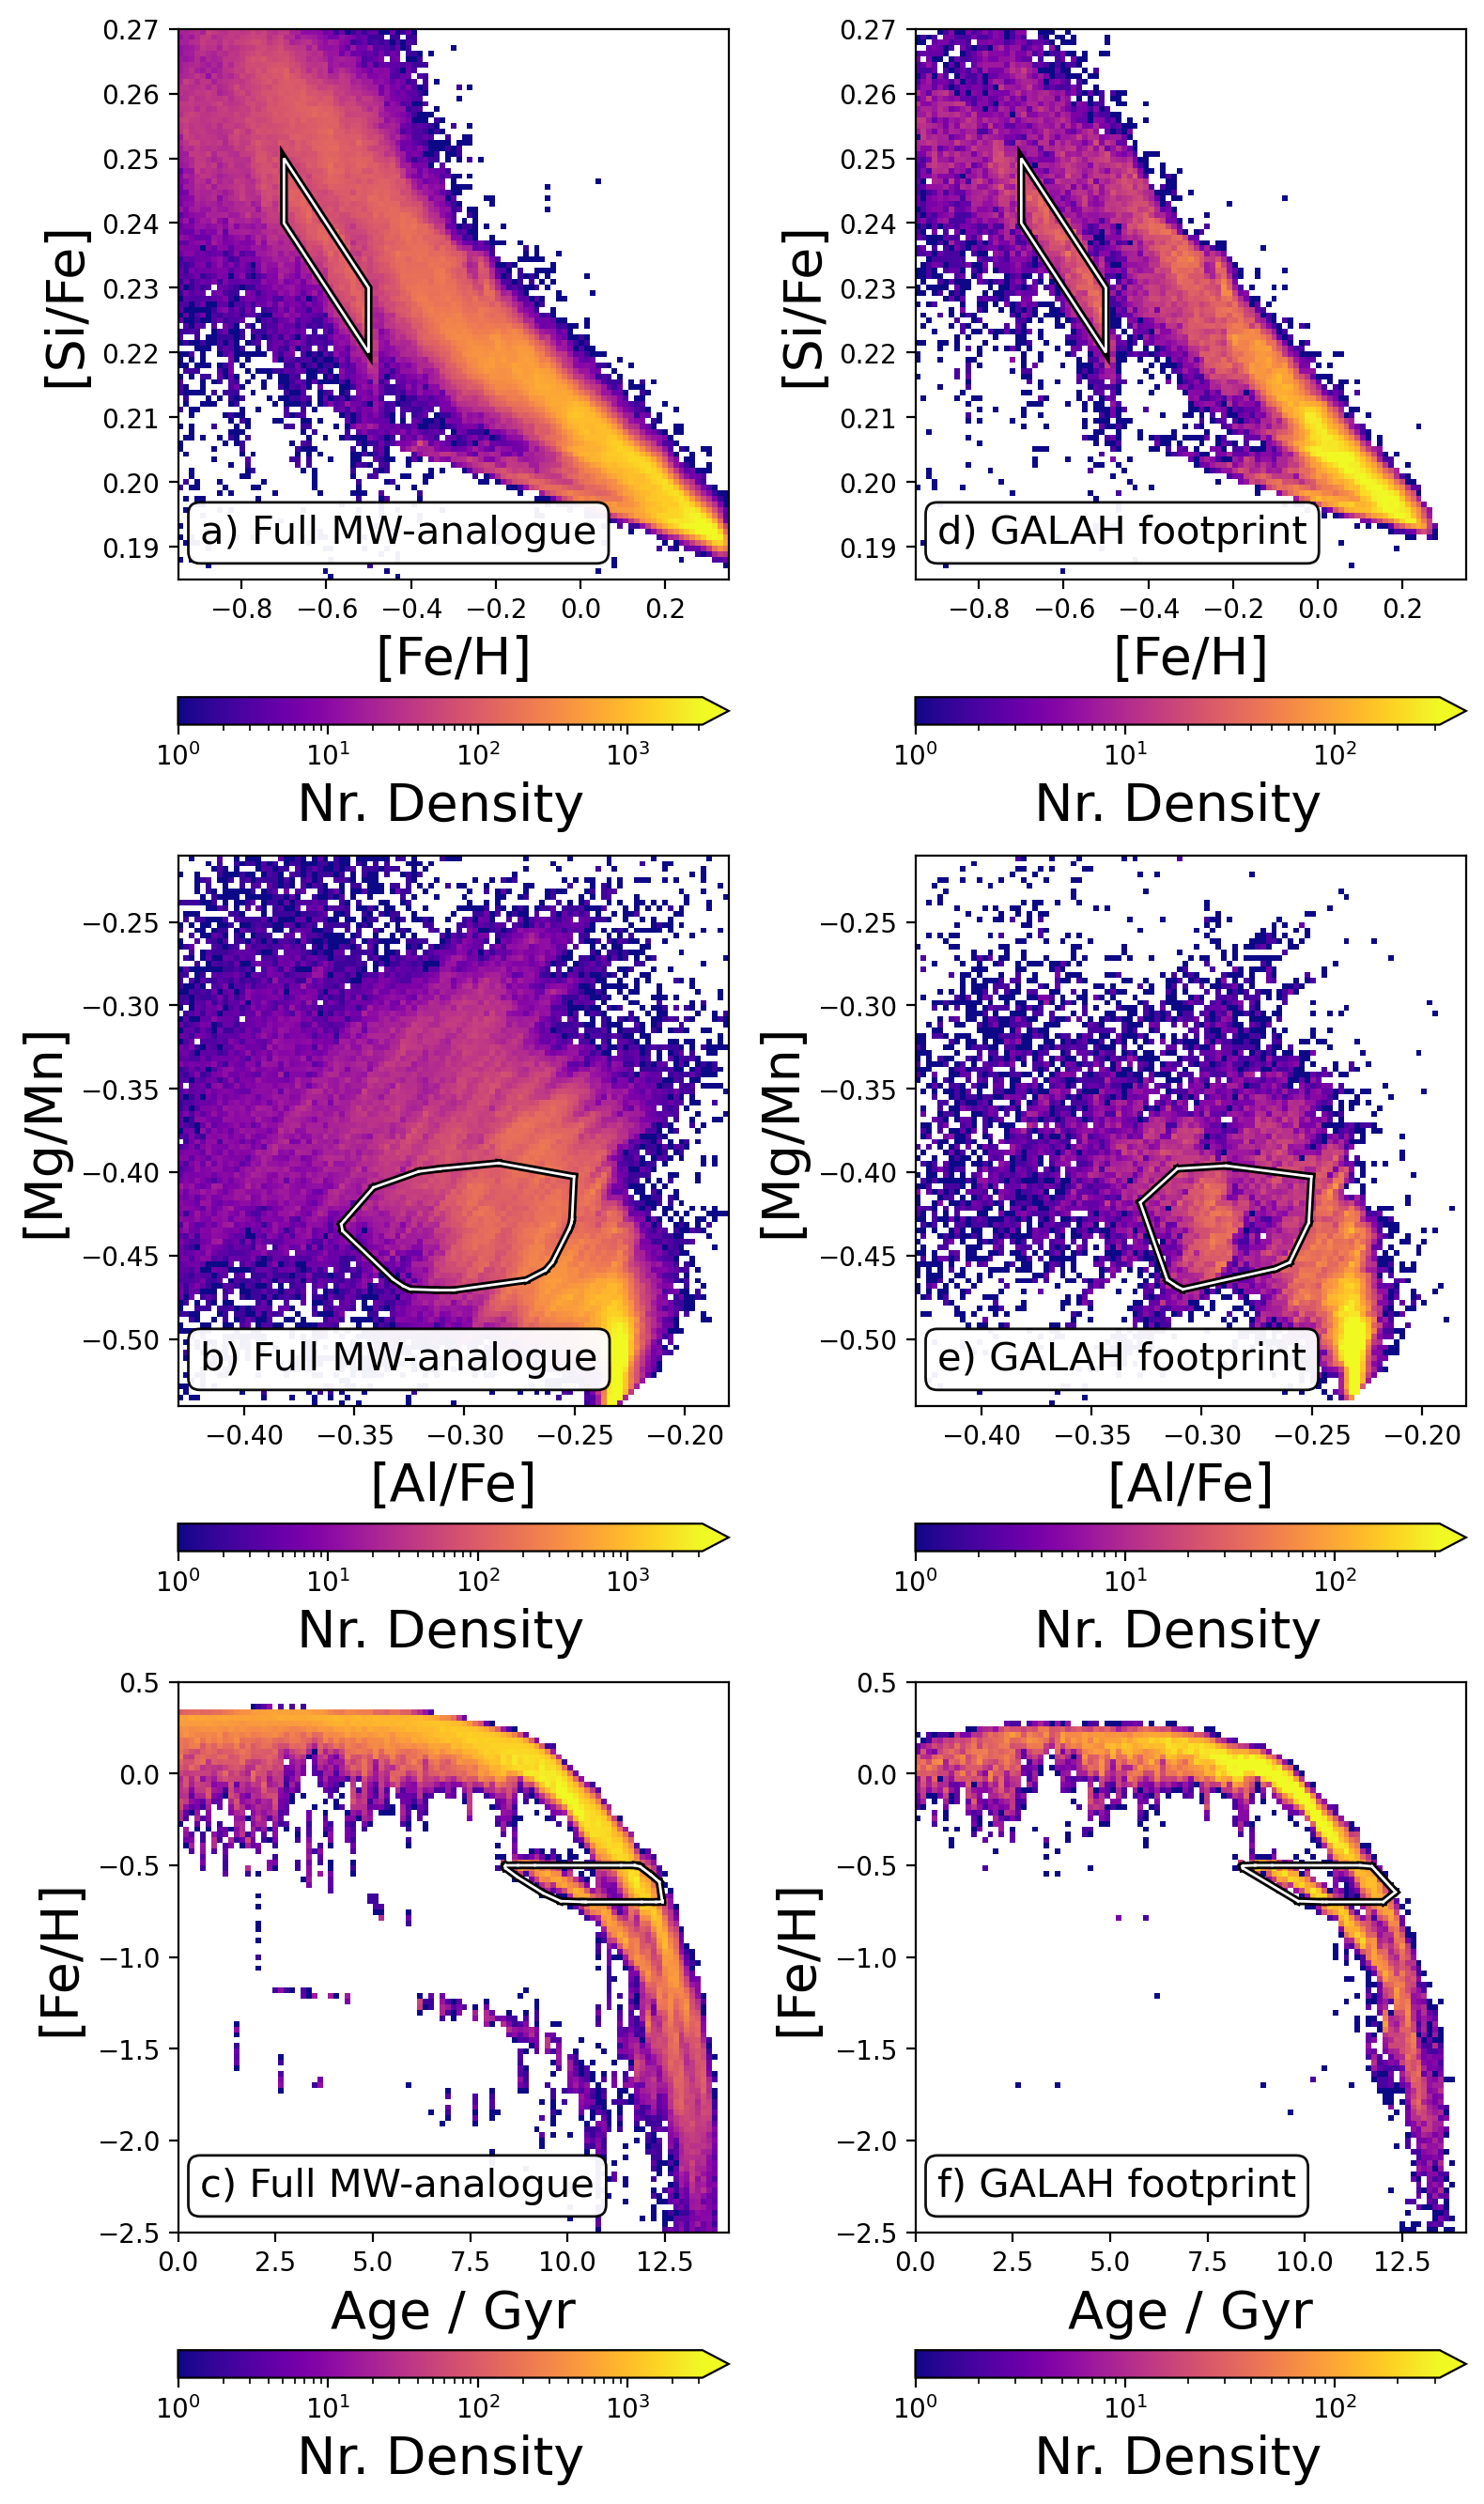
\includegraphics[width=\columnwidth]{figures/low_alpha_halo_convex_hull.png}
    \caption{
    \textbf{Density distribution of all particles (left panels) and those in a GALAH-like footprint (right panels) for particles of the NIHAO simulation \texttt{g8.26e11} (color-coded by logarithmic density).}
    \textbf{Panels a) and d):} iron vs. silicon abundances as tracers of contribution from SNIa and SNII. \textbf{Panels b) and e):} abundance combination [Al/Fe] vs. [Mg/Mn] used to trace accreted stars in observations.
    \textbf{Panels c) and f):} age-[Fe/H] relations.  
    The selection in panels a) and e) are drawn with a polygon with vertices at (-0.7,0.24),(-0.5,0.22),(-0.5,0.23), and (-0.7,0.25). A convex hull polygon of the selected stars is then drawn in other panels.}
    \label{fig:low_alpha_halo}
\end{figure}

\subsection{Location matters: Full galaxy versus Solar neighborhood} \label{sec:location}

Naïvely, we initially plot the diagnostic plots of observers, namely the ratio of SNII to SNIa via [Si/Fe] as function of iron abundance [Fe/H] in Fig.~\ref{fig:low_alpha_halo}a as well as the previously successful selection plane of [Al/Fe] vs. [Mg/Mn] in Fig.~\ref{fig:low_alpha_halo}b for the complete Milky Way analogue. In the absence of observational noise, it could be expected that areas of in-situ and accreted stars might clearly separate. To the contrary, the [Al/Fe] vs. [Mg/Mn] for the whole galaxy show seemingly even more scatter than the observations. Tracing the selection of accreted stars, that is, the stars with lower [Si/Fe] around $\mathrm{[Fe/H]} \sim -0.6$ with a selection box, does not lead to a unique location in the [Al/Fe] vs. [Mg/Mn] in Fig.~\ref{fig:low_alpha_halo}b when showing the extend of these stars with a convex hull outline.

When applying a similar selection to NIHAO as would be expected from GALAH observations in the Solar vicinity (see Sec.~\ref{sec:sim_data}), both the [Fe/H] vs. [Si/Fe] plane in Fig.~\ref{fig:low_alpha_halo}d as well as the [Al/Fe] vs. [Mg/Mn] plane in Fig.~\ref{fig:low_alpha_halo}e cleared up significantly, with the accreted sequence becoming more prominent around $\mathrm{[Al/Fe]}$ of -0.3.

\begin{figure*}
	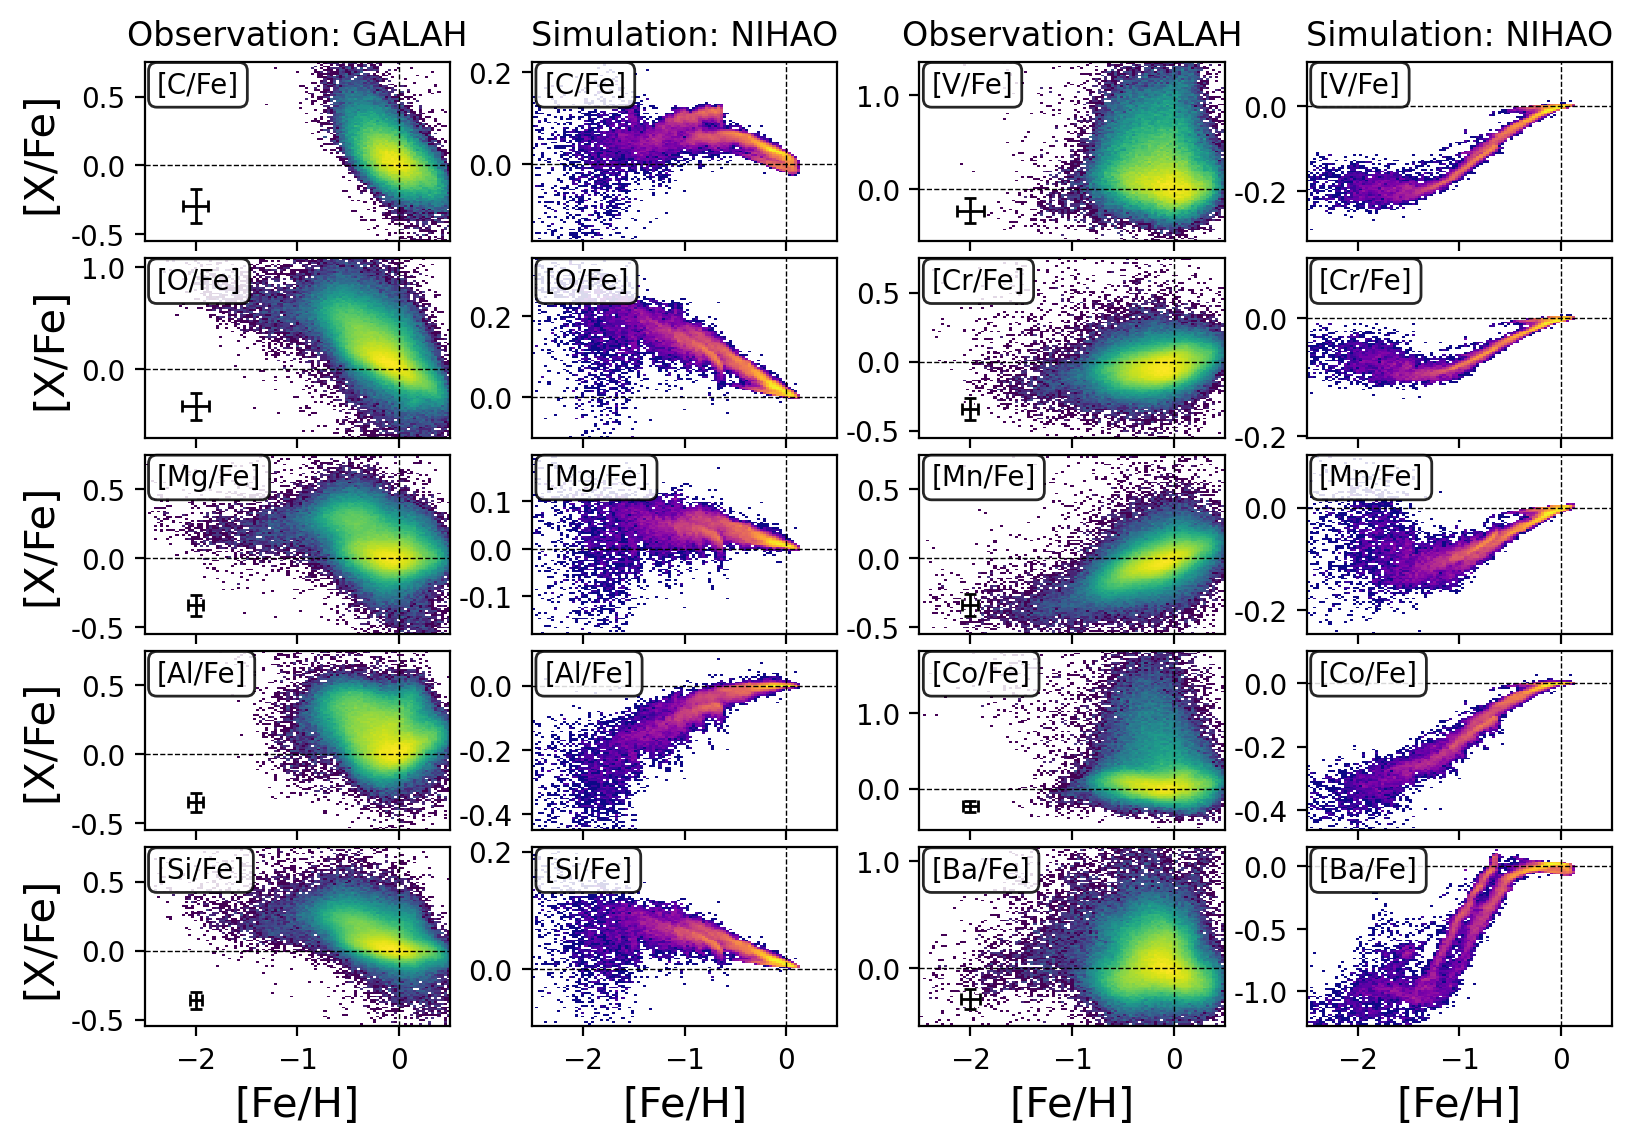
\includegraphics[width=\textwidth]{figures/Overview_FeH_XFe_Obs_Sim.png}
    \caption{
    \textbf{Logarithmic density distribution of elemental abundances [X/Fe] versus [Fe/H] for the ten elements overlapping between GALAH and NIHAO.} 
    \textbf{First and third rows} show observed data from GALAH while \textbf{second and fourth rows} show the simulated data for the same abundance ratios in a GALAH-like footprint. Brighter colors (towards yellow) indicate higher densities. For better visibility, plot ranges are adjusted to the data rather than to be equal among each panel. Dashed lines indicate Solar values.}
    \label{fig:FeH_XFe}
\end{figure*}

Intrigued by the difference in clarity of the chemical planes, we also show the two age-metallicity relations - or more accurately age-[Fe/H] planes - for the full Milky Way analogue in Fig.~\ref{fig:low_alpha_halo}c and the observational footprint in Fig.~\ref{fig:low_alpha_halo}f. The clearly arising separations of sequences in both selections motivates a more dedicated analysis of this plane, as will follow in Sec.~\ref{sec:Age-abundance}. Under this section's theme of identifying differences in the planes of full and limited sample selection, we notice a slightly larger scatter of abundances in Fig.~\ref{fig:low_alpha_halo}c, that is, a differences of iron abundances outside the Solar vicinity, as well as the disappearance of a metal-poor ($\mathrm{[Fe/H]} \sim -1.5$) sequence below $10\,\mathrm{Gyr}$ when limiting the selection to the GALAH footprint.

\textbf{Key Takeaway:} Location matters, or better: a clever sample selection - even for simulations!

\subsection{Abundance trends: [Fe/H] vs. [X/Fe]} \label{sec:feh_xfe}

In Fig.~\ref{fig:FeH_XFe}, we show the elemental abundances [X/Fe] as a function of iron abundance [Fe/H] of the 10 elements X that overlap between GALAH observations and NIHAO simulations. To first order we see an agreement of general trends for most elements, that is, elements that are produced by CC-SN like O, Mg, and Si are showing a high plateau for low [Fe/H] and a decrease towards higher iron abundances - as expected by the onset of Fe-producing SNIa. The iron-peak elements Cr as well as Mn and Co show increasing abundances from low values at low [Fe/H] towards solar values at solar [Fe/H]. Abundance estimates for V and Co do not agree, which is partially (but not fully) caused by unreliably high measurements of [V/Fe] and [Co/Fe] in GALAH \citet{Buder2021}. For Ba, we note tightly increasing enhancements towards Solar [Fe/H], starting from initially low values around $\mathrm{[Ba/Fe]} \sim -0.5$. Furthermore, we notice a clear second (accreted) sequences below $\mathrm{[Fe/H]} < -0.5$ for C as well as Ba. While not shown in this manuscript, we note that when plotting the full simulated galaxy in Fig.~\ref{fig:FeH_XFe}, no significant difference in trends can be identified, but a larger spread of abundances - most notably towards the lowest metallicities.

When focusing on the actual absolute abundances (note the difference in y-axis), we note significant differences between the chemical evolution sequences. To understand this difference, we first need to remind ourselves that the observational data is limited by the ability to measure abundances (note the missing abundances of [C/Fe] for low metallicities due to detection limits) and includes measurement noise, while the theoretical data does not necessarily have to reproduce the formation scenario of the Milky Way and chemical enrichment tracing is limited to our best current understanding of nucleosynthesis, see e.g. the discussion of nucleosynthetic yields in \citet{Buck2021}.

That said, we note that none of the abundance sequences in the Solar metallicity regime of $\mathrm{[Fe/H]} \sim 0$ intercept with the expected Solar value. While C, O, Si, Cr, Mn, and Ba are significantly overproduced between $0.05$ (for Cr) and $0.5\,\mathrm{dex}$ (for Ba), we notice a significant under-abundance on the $-0.3..-0.1\,\mathrm{dex}$ level for Mg, Al, V, and Co.

\textbf{Key Takeaway:} While simple abundance-metallicity plots do not easily reveal accreted structures for most elements, both C and Ba abundances show the potential to identify different abundance sequences - if the nucleosynthetic processes of the simulation are accurate.

\subsection{Abundance-abundance plots: [Al/Fe] vs. [Mg/Mn]} \label{sec:alfe_mgmn}

We now turn then to abundance-abundance plots of [Al/Fe] vs. [Mg/Mn] that were already mentioned in Sec.~\ref{sec:location}. These plots combine the enrichment channels of CC-SN vs. SNIa, that is [Mg/Mn], and the enrichment of Al with more complex metallicity-dependent enrichment pathways \citep{Hawkins2015, Das2020, Kobayashi2020}. The enhancements of these elements should differ significantly when comparing in-situ stars born in the early Milky Way with the less massive system that it accreted because of the expected lower star formation intensity (and thus iron abundance) and occurrence of CC-SN in the latter. 

\begin{figure}
	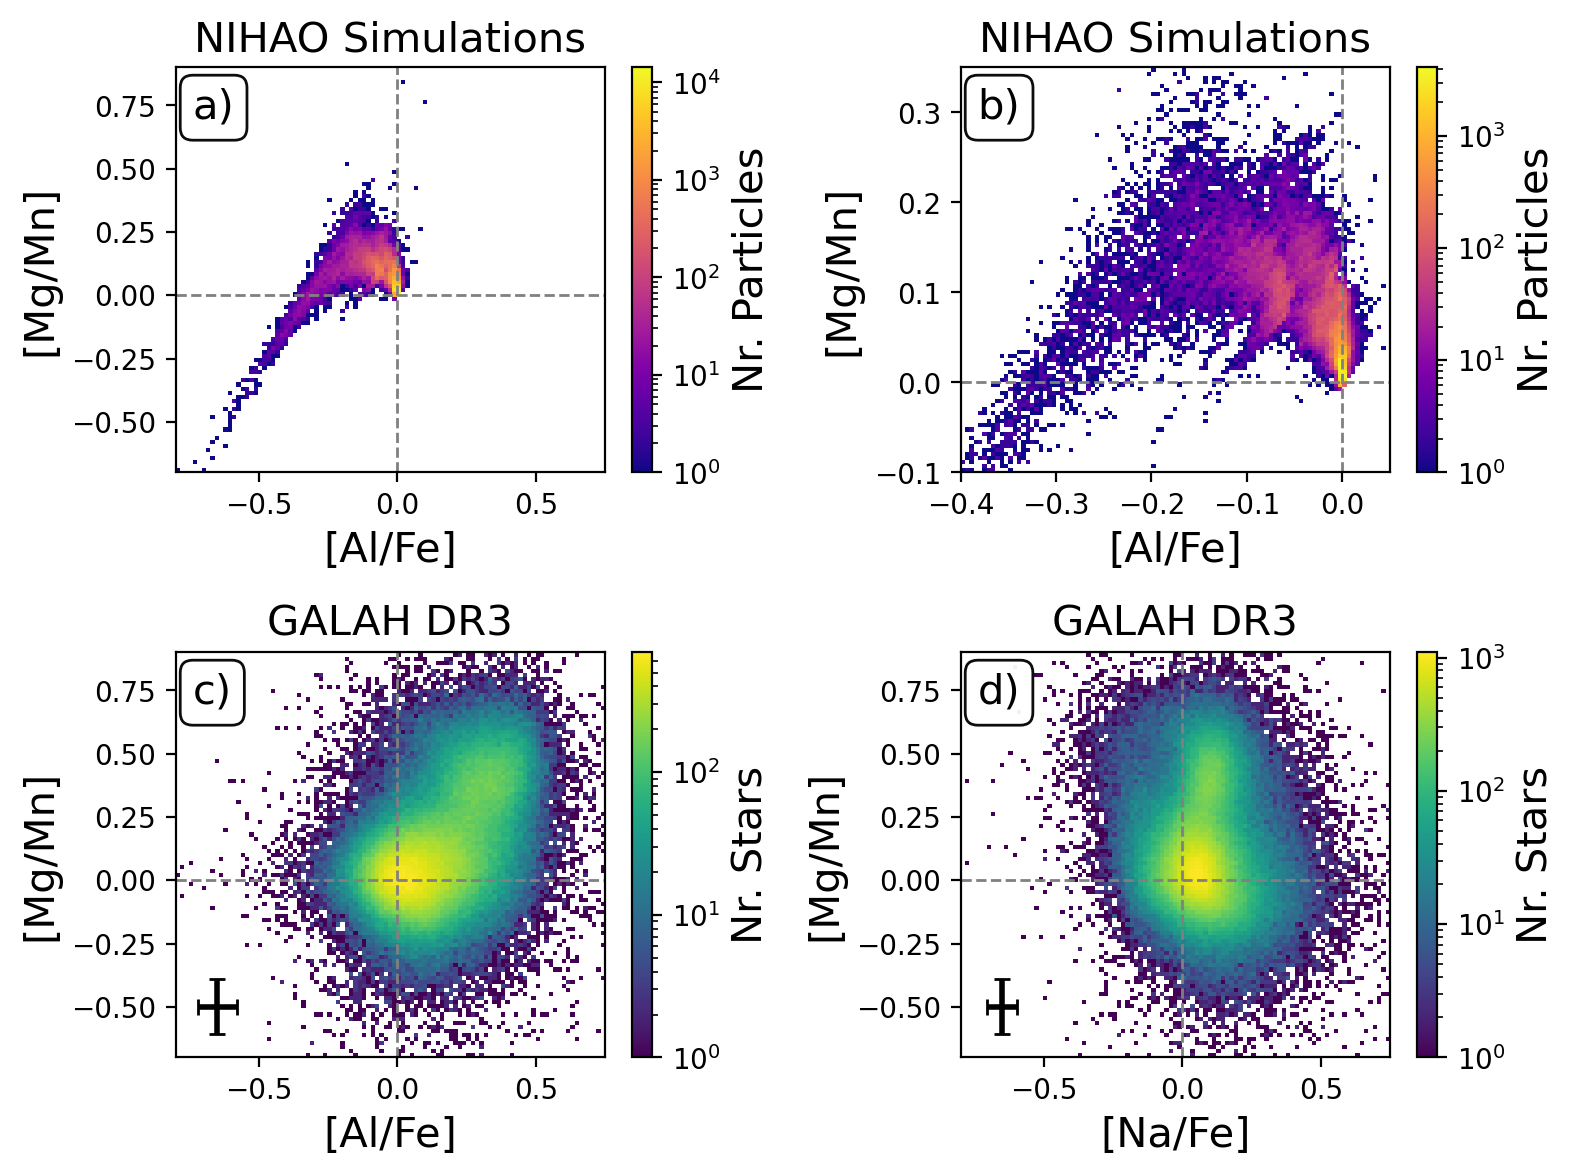
\includegraphics[width=\columnwidth]{figures/mgmn_alfe.png}
    \caption{
    \textbf{Comparison of the diagnostic plot of odd-Z elements [Al/Fe] or [Na/Fe] vs. the ratio of CC-SN and SNIa elements [Mg/Mn] in simulation (top) and observation (bottom), with accreted stars being expected in the upper left of the distributions.}
    \textbf{Left panels a and c} use the same axis limits, whereas \textbf{panel b} is a zoomed version of the simulation. \textbf{Panel d} complements the picture, as [Al/Fe] is hard to measure in GALAH (see missing data points in top left of panel c).
    }
    \label{fig:NaFe_MgMn_selection_Age_FeH_dissection}
\end{figure}

When using the same axis limits for simulation and observation (Figs.~\ref{fig:NaFe_MgMn_selection_Age_FeH_dissection}a and c), we notice the strong offset and significantly smaller spread of abundances in the simulation, in agreement with our previous findings for abundances in Sec.~\ref{sec:feh_xfe}. When zooming into the relevant [Al/Fe] vs. [Mg/Mn] regime for the simulations, however, we notice a better qualitative agreement, in that we see two significant overdensities for simulated and observed galaxy. For the observations, we identify the lower and upper overdensity at [Mg/Mn] of 0.0 and 0.4. These have previously been confirmed as low- and high-$\upalpha$-sequence (or thin and thick disk), respectively \citep{Hawkins2015, Buder2022}. These sequences show similar Solar or even enhanced [Na/Fe] and [Al/Fe]. In contrast to this, the major overdensity in the simulation is found around (-0.25,-0.5) with tails reaching higher [Mg/Mn]. The minor overdensity is found towards higher [Mg/Mn] as well as lower [Al/Fe] - coinciding with the expected region of accreted stars \citep{Horta2021} which are less numerous in the observational data of GALAH DR3.

\textbf{Key Takeaway:} The abundance-abundance plot of [Al/Fe] vs. [Mg/Mn] show qualitative agreement with the observational data, but with significant abundance offsets and a more pronounced overdensity of accreted stars than the observations. This could indicate a more massive merger progenitor than the Milky Way's GSE or hint at our inability to actually measure Mg, Mn, and Al or Na abundances of accreted stars.

\section{A new (?) angle: age-abundance-distributions}\label{sec:Age-abundance}

Fortunately, chemistry is not the only conserved property of stars. We therefore turn to stellar ages and assess age-abundance trends in the data, starting from the age-[Fe/H] relationship that we already showed in Figs.~\ref{fig:low_alpha_halo}c and f. This relation has proven to be a powerful tool not only for resolving processes with observed data of our Milky Way \citep[e.g.][]{Twarog1980, Edvardsson1993, Nordstroem2004, Casagrande2011, Feuillet2019, Xiang2022}, but also other galaxies - for example to identify accreted stars \citep[e.g.][]{Pinna2019b, Martig2021}. However, observations still suffer from incredibly large uncertainties on the order of $15-50\%$ for most stars, so examining simulation plots removes this barrier and allow us to determine chemical enrichment as a function of age.

\subsection{Clearly separated sequences in the age-[Fe/H] relation of the Milky Way analogue} \label{sec:sequences}

Based on Fig.~\ref{fig:low_alpha_halo}f, we identify two definite and one tentative sequence in the age-metallicity relation with the following selections, selecting 74\,129 particles for Sequence 1, 9\,813 particles for Sequence 2, and 2\,085 particles for Sequence 3 of the 88\,980 particles in the footprint%
:
\begin{align}
    \text{Sequence~1} &= \begin{cases}
        \mathrm{[Fe/H] > -0.2} \text{ or} \\
        (\mathrm{[Fe/H]} > -1.0 \text{ and } \mathrm{age} < 7\,\mathrm{Gyr}) \text{ or} \\
        10^{\mathrm{[Fe/H]} + 0.2} > 2.0 - 0.15*\mathrm{age}~/~\mathrm{Gyr}
    \end{cases} \label{eq:sequence1} \\
    \text{Sequence~2} &= \begin{cases}
        \text{Not Sequence~1 and }\mathrm{Age} > 6\,\mathrm{Gyr} \text{ and} \\
        10^{\mathrm{[Fe/H]} + 0.3} > 1.87 - 0.15*\mathrm{Age}~/~\mathrm{Gyr}
    \end{cases}  \label{eq:sequence2} \\
    \text{Sequence~3} &= \text{Not Seq.~2 and not Seq.~3 and } \mathrm{age} > 7~/~\mathrm{Gyr}  \label{eq:sequence3}
\end{align}

\begin{figure*}
	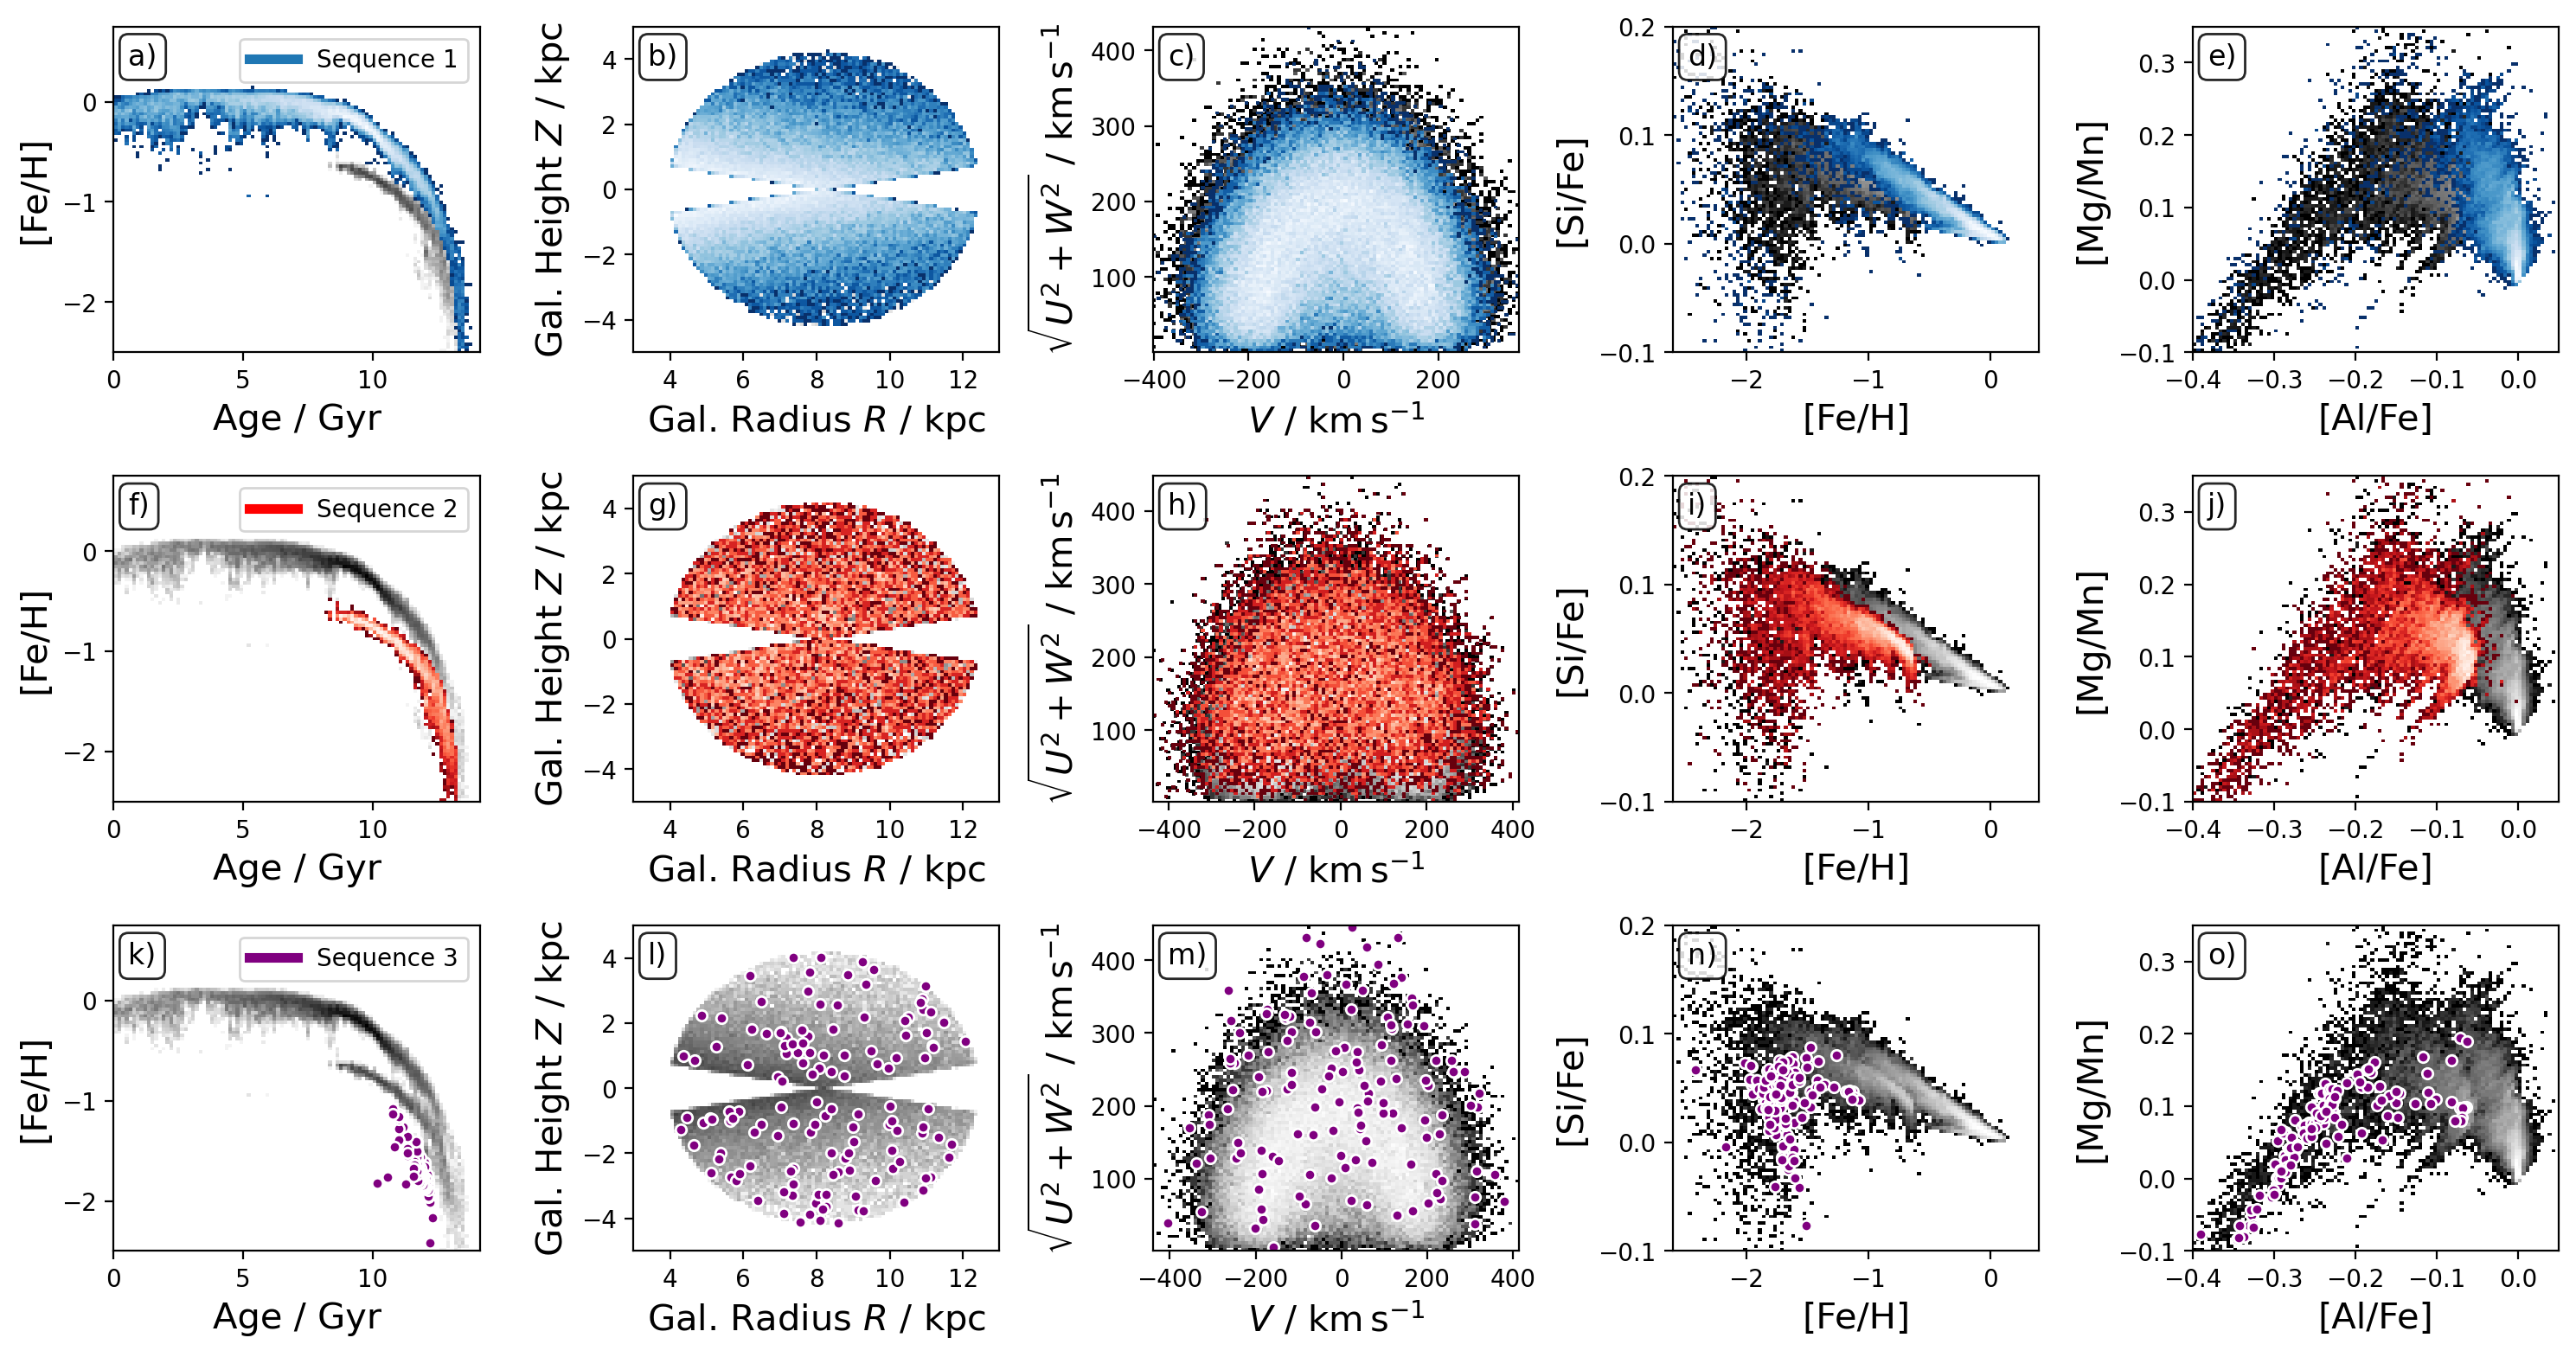
\includegraphics[width=\textwidth]{figures/three_sequences_traced.png}
    \caption{
    \textbf{Chronochemodynamic properties of the three separate sequences identified in the age-[Fe/H] relation (first column) - blue for Sequence 1 in the top row, red for Sequence 2 in the middle row, and purple for Sequence 3 in the bottom row.
    }
    \textbf{The second column} shows the spatial density of stars in $R$-$z$.
    \textbf{The third column} shows the kinematic extend of stars in the Toomre diagram of $V$ vs. $\sqrt{U^2+W^2}$.
    \textbf{The fourth and fifth columns} show chow the chemical distribution in the [Fe/H] vs. [Si/Fe] and [Al/Fe] vs. [Mg/Mn] plane, respectively.
    }
    \label{fig:three_sequences_traced}
\end{figure*}

In Fig.~\ref{fig:three_sequences_traced}, we trace three sequences in separate rows in their chronochemodynamic properties, starting with the age-[Fe/H] relation.

For Sequence~1, the most metal-rich sequence with 83\%%
 of particles in the footprint, we see the stars being distributed closest to the galactic plane ($\vert Z \vert < 2\,\mathrm{kpc}$) in Fig.~\ref{fig:three_sequences_traced}b. Their kinematics in Fig.~\ref{fig:three_sequences_traced}c) likens a Toomre diagram of the Milky Way thin and thick disk \citep[][see their Fig.~1a]{Helmi2018} that is mirrored around $V$ (as could be expected given our 3-dimensional selection of a torus rather than a sphere.


$\,$
\SB{CONTINUE HERE}
\\ $\,$

age-metallicity relation (first column), their spatial distribution (second column), their kinematic distribution (third column), as well as their chemical distributions (fourth and firth columns).


Fig.~\ref{fig:three_sequences_traced}a-d showing Sequence 1, Fig.~\ref{fig:three_sequences_traced}e-h showing Sequence 2, and Fig.~\ref{fig:three_sequences_traced}i-l showing tentative Sequence 3.








Although the observational plots showed incomprehensible results, there is very clear substructure in the simulated age-abundance plots, with two distinct streams for the two populations (in-situ and accreted). The comparison of observed and simulated age-abundance plots is shown in Figs \ref{fig:BaFetime} and \ref{fig:BaHtime}. The top stream in the plots is likely representative of the in-situ population, as we know that accreted populations tend to join the Milky Way from smaller galaxies with less massive stars. This means that the stars are less metal-heavy and explains the lower stream of accreted stars that can be observed in the simulation data.

The stark difference in clarity of results between the uncertainty-free simulation data and the high-uncertainty GALAH data highlights the importance of reducing observation noise, and provides clear motivation for further investigation into these plots as diagnostic tools. Similar plots have been used already with GALAH data to identify accreted substructure in galaxies other than the Milky Way \citep{Martig2021}.

\textbf{Key Takeaway:} Age is a conserved characteristic of stars that shows distinct populations when plotted against chemical abundance.

\begin{figure}
	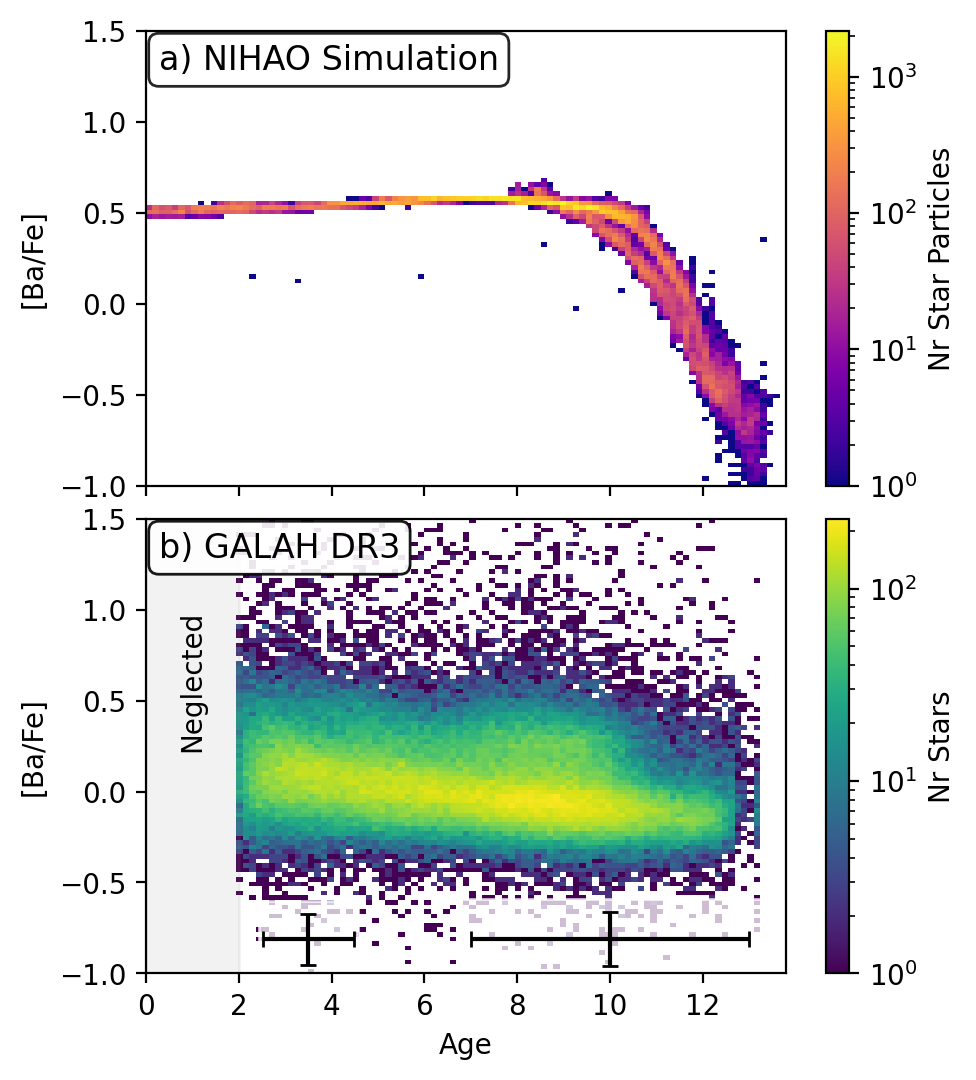
\includegraphics[width=\columnwidth]{figures/Ba_Fe_time.png}
    \caption{Barium abundance in a ratio with Iron [Ba/Fe] as a function of age. Simulation data (top) and GALAH data (bottom) shows clear differences in scatter. Although not entirely separate, it is clear that there are two different overdensities in a 'stream'-like shape.}
    \label{fig:BaFetime}
\end{figure}
\begin{figure}
	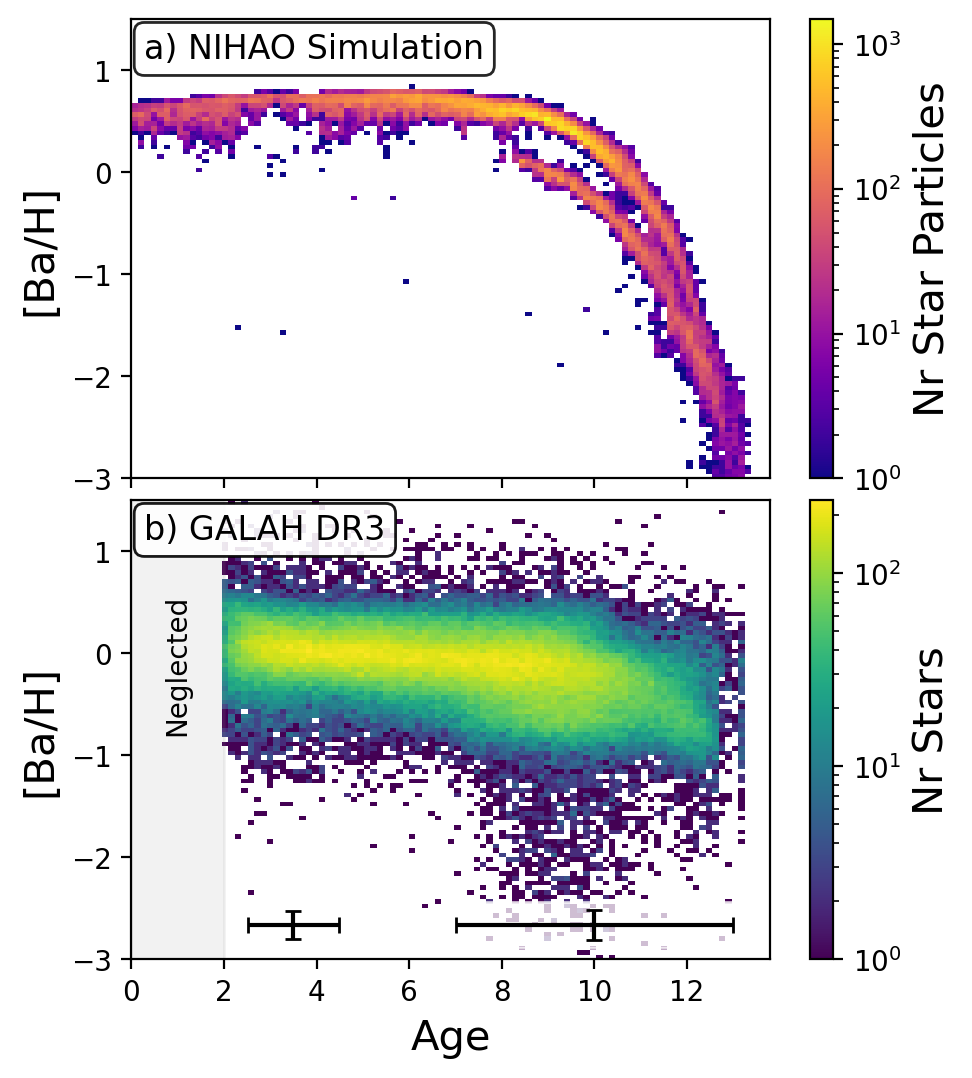
\includegraphics[width=\columnwidth]{figures/Ba_H_time.png}
    \caption{Simulation (top) vs observation (bottom) plots of Barium's evolution with age, with Ba plotted in a ratio against H instead of Fe. The top stream represents the in situ stars, while the lower stream is stars that have since accreted and hence follow a similar evolution path but at lower element abundances.}
    \label{fig:BaHtime}
\end{figure}
\begin{figure}
	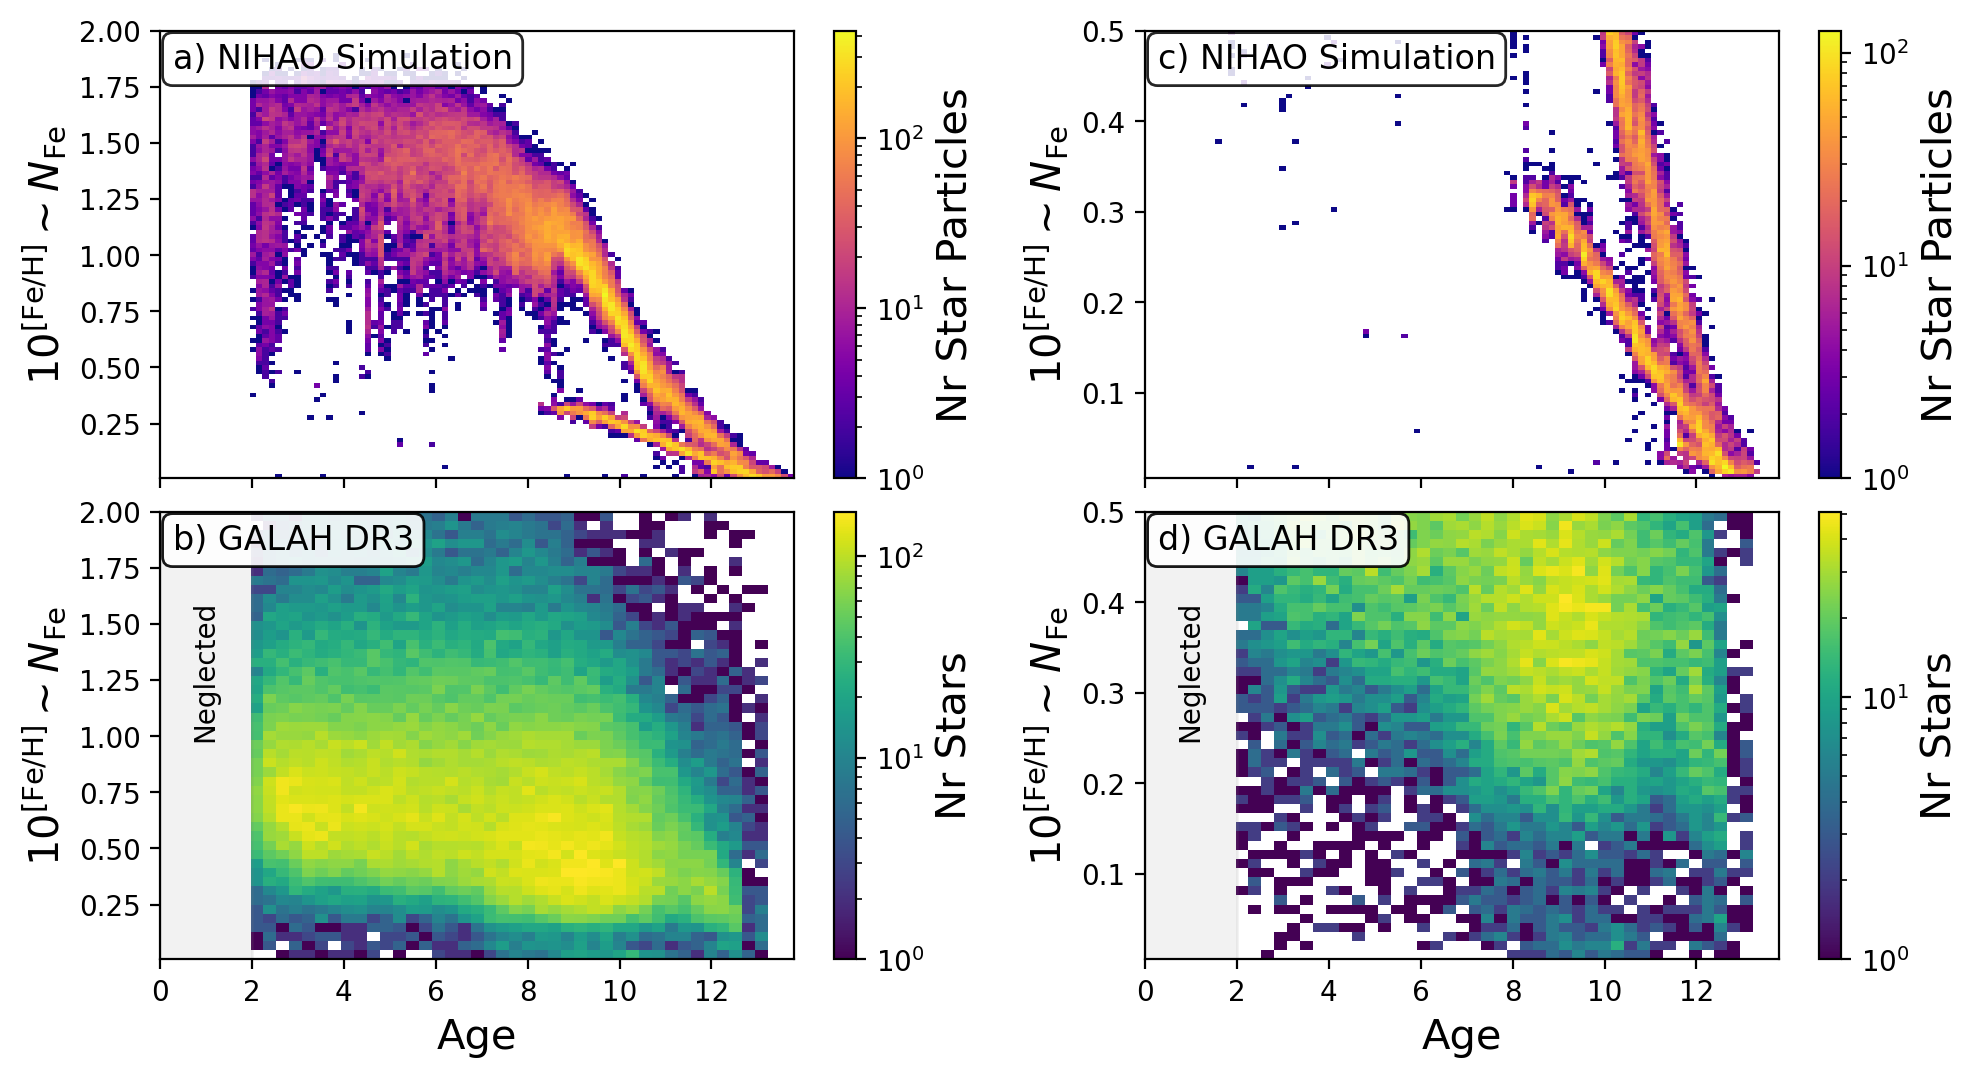
\includegraphics[width=\columnwidth]{figures/Fe_H_lin_time.png}
    \caption{Age-metallicity relation in logarithmic and linear space.}
    \label{fig:Fe_H_lin_time}
\end{figure}

\subsection{The importance of notation: [X/Fe] or [X/H]}
Several existing studies have suggested using elemental abundances reported as a function of Hydrogen number density (\citet{Fuhrmann2017}, \citet{Feuillet2021}). We produced the age-abundance plots using a range of chemical abundances, and confirmed this finding— that [X/H] produced the most clarified plots. This is highlighted in Figures \ref{fig:BaFetime} and \ref{fig:BaHtime} where we compare age plots of [X/Fe] and [X/H], and see much more clearly separated stellar populations in the H plot. Fe is being simultaneously enriched along with the element we are comparing it to (Ba is used here as an arbitrary example), which results in less clarity in the overall plot. As Hydrogen was formed in the Big Bang nucleosynthesis, it is not enhanced or affected by time in the same way that metals like Fe are. Having determined the most suitable plot for identifying accreted populations via the simulations, it is now important to consider the problem from a realistic perspective, and quantitatively determine how much noise we could allow for both abundance and age estimates to still be able to separate the sequences. \par 

\SB{Note interesting facts in Fig.~\ref{fig:Fe_H_lin_time}:
\begin{itemize}
    \item Clear separation in sequences
    \item Linear increase of accreted stars.
    \item Onset of chemical scatter for in-situ stars of simulation coincides with end of star formation in accreted sequence (compare with Lucy's work!)
    \item Gap in stars also in observable space. Where are the GSE stars? 0.3 or below 0.1?
\end{itemize}
}
% \begin{itemize}
%     \item Discuss that some previous studies have suggested to use elemental abundances reported as a function of hydrogen number density \citep[see e.g.][]{Fuhrmann2017b, Feuillet2021}.
% \end{itemize}

% Fig.~\ref{fig:BaHtime} shows the elemental ratio of [Ba/Fe] over time. This same plot was created using every elemental combination available in the dataset, and it was found that the combination of [X/H] over time produced the clearest plot, as in Fig.~\ref{fig:BaHtime}. Hydrogen, being formed in the Big Bang nucleosynthesis, is not enhanced or affected by time, whereas metals like Fe are. This is why [X/H] plots are decidedly clearer than [X/Fe], as Fe is being simultaneously enriched along with Ba.

% As the abundances show clear sequences in [Ba/H] (and the other abundances), we now want to study how much noise we could allow for both abundance and age estimates, to still be able to separate the sequences.
\par\textbf{Key Takeaway:} The abundance vs age plots are clearest when the abundance is relative to H, rather than Fe or any other metal.


\subsection{Quantifying differences of age-abundance sequences} \label{sec:ageabundance}

To determine two different stellar populations as being accreted and in situ, we need to be able to quantify the difference between the two groups. This is done using separation significance $r$. This value is found using Eq.~\ref{eq:r_value}, which has been adapted from \citet{Lindegren2013}, and assumes a Gaussian distribution around a mean value $\mu$ with a standard deviation $\sigma$, for each population. This assumption is confirmed by plotting a histogram of [X/H] for the simulation between 8 and $9\,\mathrm{Gyr}$, an example of which is found in Fig.~\ref{fig:hist_labels}. The larger peak (with subscripts of 2) represents the in-situ population, and the smaller (1) is the accreted population. 

\begin{equation} \label{eq:r_value}
r = \frac{|\mu_1 - \mu_2|}{\sqrt{\sigma_1^2 + \sigma_2^2}}
\end{equation}

In the simulation the standard deviation would only incorporate the intrinsic scatter, that is, $\sigma_{1,\text{obs}} = \sigma_1$. In the observations, the observational scatter (which we assume uniform throughout the parameter space) would enter into Eq. \ref{eq:r_value} via
\begin{equation} \label{eq:scatter}
    \sigma_{1,\text{obs}} = \sqrt{\sigma_1^2+\sigma_{obs}^2},
\end{equation}
leading to a slightly adjusted version of Eq.~\ref{eq:r_value}, that is,
\begin{equation} \label{eq:r_value_observed}
r (\sigma_{obs}) = \frac{|\mu_1 - \mu_2|}{\sqrt{\sigma_1^2 + \sigma_2^2 + 2\cdot \sigma_{obs}^2}}.
\end{equation}

\begin{figure}
	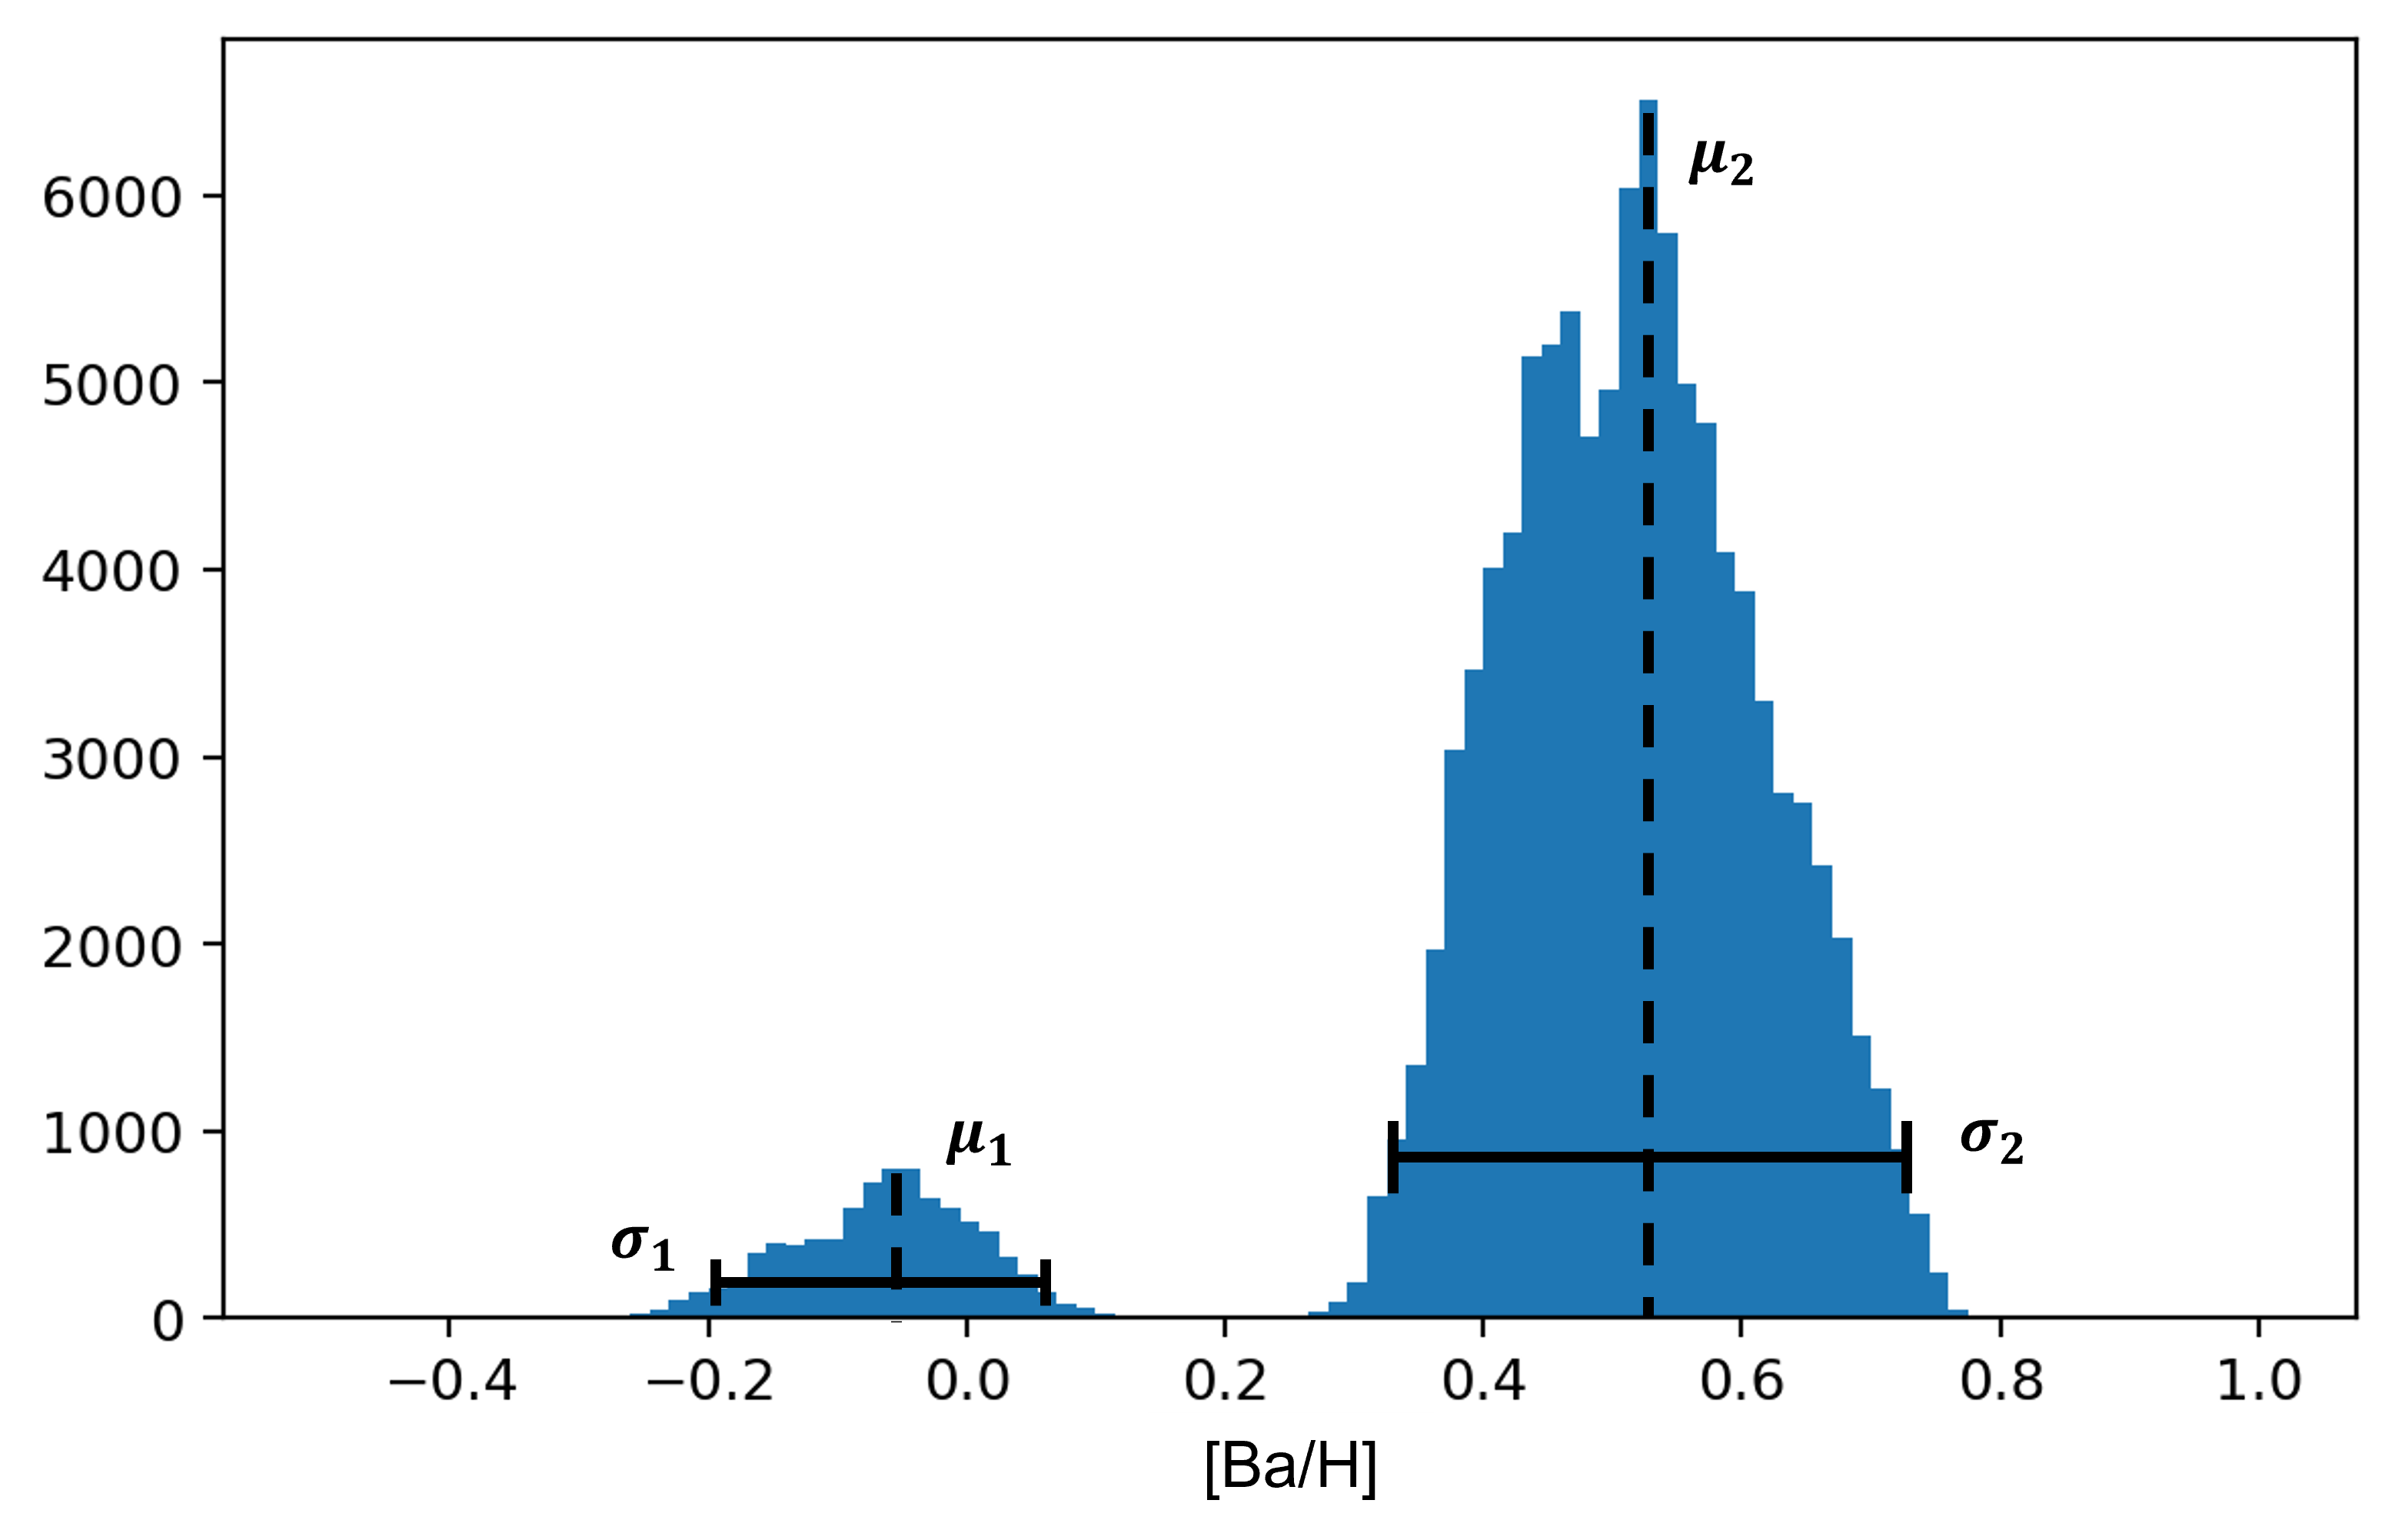
\includegraphics[width=\columnwidth]{figures/hist_labelled.png}
    \caption{A discrete 1D histogram of Barium (used just as an example), with two distinct Gaussian distributions representative of the accreted and in situ populations. This plot has been labelled with diagramatic indicators of the values of mean ($\mu_1$ and $\mu_2$) and standard deviation ($\sigma_1$ and $\sigma_2$) which are used in this project to quantify the separation between populations.}
    \label{fig:hist_labels}
\end{figure}

To determine the positions of the sequences and subsequent separation of data, we fit a bimodal Gaussian model to the data, for each element. These values are tabulated in Table.~\ref{tab:r_values_simulation}, along with the calculated r-value.\par 

\textbf{Key Takeaway:} The data is in the form of a Gaussian model, which could be used to determine the standard deviations and means of both populations, and quantify the separation significance. 


% We then split the dataset for this particular into 2 and calculated 16th, 50th, and 84th percentiles in order to recover a more robust mean and standard deviation (and monitor our assumption of a Gaussian distribution).
% \SB{We list the values of 16th, 50th, and 84th percentiles as well as the resulting $r$ values in Tab.~\ref{tab:r_values_simulation}.}

\begin{table}
    \centering
    \caption{Separation significance for the simulated data between in-situ and accreted (accr.) sequences for abundances ratios [X/H] of ten elements X.}
    \begin{tabular}{cccccc}
    \hline
    Element & $\mu_\text{in-situ}$ & $\sigma_\text{in-situ}$ & $\mu_\text{accr.}$ & $\sigma_\text{accr.}$ & $r$\\
    \hline \hline
    {[C/H]}  & 0.0 & 1.0 & 0.0 & 1.0 & 5.3 \\
    {[O/H]}  & 0.0 & 1.0 & 0.0 & 1.0 & 5.3 \\
    {[Mg/H]}  & 0.0 & 1.0 & 0.0 & 1.0 & 5.3 \\
    \hline
    \end{tabular}
    \label{tab:r_values_simulation}
\end{table}
 % \label{tab:r_values_simulation}

\subsection{Assessing the influence of observational uncertainties}

Having identified age-abundance plots as the clearest diagnostic tool of accreted stars, and having quantified our results, we now seek to determine what uncertainty limit is acceptable in our observations. We do this two-fold. Firstly, we test how much observational scatter $\sigma_{obs}$ is allowable, while still being able to tell apart the sequences with a confidence of 68\% or 95\% (r-values of at least 1 or 2). This is plotted in Fig.~\ref{fig:r_v_obs}, and quantified in Table \ref{tab:r_values_simulation}. It is clear that all elements have a relatively similar error allowance of 0.18 for 95\% confidence and 0.38 for 68\%. Comparing these values to GALAH data used in this study finds that most measured element uncertainties, but not all, fall below our calculated threshold. \par  
We then must consider the second facet of uncertainty: the age uncertainties of the data. We expect the sequences will be significantly more difficult to distinguish in older stars with corresponding larger uncertainties. This is plotted in Fig.~\ref{fig:r_v_age}, using a subset of data within 4-5Gyr. This age subset is used as it is the range within which there is the clearest separation between the two populations in the simulated plots, shown in Figs. \ref{fig:BaFetime} and \ref{fig:BaHtime}. We see there is more deviation among elements than in Fig.~\ref{fig:r_v_obs}, but there remains a similar cut-off point where separation significance increases notably, at approximately 1Gyr. Because we are working within the age range of 4-5Gyr, this means that a 1Gyr uncertainty is equivalent to just over 20\%. We can see from the plot that we require an uncertainty of around 15\% before the r-value begins to increase, which is much lower than the age uncertainties we currently have from GALAH data. \par
\textbf{Key Takeaway:} We are able to quantify the level of uncertainty (both in element and age measurements) allowable for clear populations, and find the GALAH data has sufficient element measurements, but significantly too high age uncertainties. 



% \begin{itemize}
%     \item abundances uncertainties, entering as $\sigma_{\text{obs}}$ into Eq.~\ref{eq:r_value_observed}.
%     \item age uncertainties, making it hard to distinguish between the sequences for the oldest stars.
% \end{itemize}

% Assessing both influences in the observational data is difficult because we do not know the underlying distribution of accreted versus in-situ stars. We therefore turn to the simulations and perform two tests. Firstly, we test how much observational scatter $\sigma_{\text{obs}}$ is allowed to still tell apart the sequences with a confidence of 68 or 95\% ($r$-values of at least 1 or 2)? Secondly, we test how well we can tell the sequences apart when adding age uncertainties. In this particular case, we start from our initial subset selected for ages of $8-9\,\mathrm{Gyr}$ and ask, how would our selection change, if we cannot separate these stars from the even older ones (increasing our selection from $8-9\,\mathrm{Gyr}$ towards $8-10\,\mathrm{Gyr}$, $8-11\,\mathrm{Gyr}$, etc.)?

% We plot the results of the first test, $r (\sigma_\text{obs})$ in Fig.~\ref{fig:r_v_obs} and compare it to the average reported uncertainty from GALAH. There is very little range between elements on these plots, and it is clear that all elements require a level of noise to be below approximately 0.4 to be 68\% sure the populations are separate, and below 0.2 to be 95\% confident. Within the accessible GALAH dataset, we can access the corresponding measurement uncertainties, and find that most, but not all, measurements of chemical abundances fall below these thresholds - if they can be measured and are reported.

\begin{figure}
	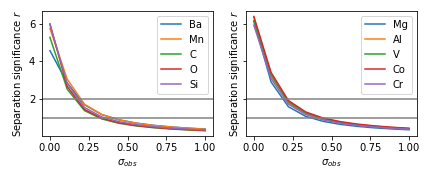
\includegraphics[width=\columnwidth]{figures/same_axis_r_sigma.png}
    \caption{Similar to Fig.~\ref{fig:r_v_age}, this plot shows all elements on an axis of their separation significance $r$ as a function of measurement noise. There are two horizontal lines at $r=1$ and $r=2$ which show the points at which we can be 68\% and 95\% confident (respectively) that we are observing two distinct populations. It is clear that these values are quite similar for all elements.}
    \label{fig:r_v_obs}
\end{figure}

\begin{table}
    \centering
    \caption{Observational uncertainties for each element that allow to separate the in-situ and accreted sequences at $8-9\,\mathrm{Gyr}$ with 95\% ($r>2$) and 68\% ($r>1$) certainty. The last rows report the percentage of measurements and their the median uncertainties for the element reported by GALAH DR3 (as indicators of how often and how well the element can be measured.}
    \begin{tabular}{ccccc}
    \hline
    Element & $\sigma_\text{obs}$ 95\% & $\sigma_\text{obs}$ 68\% & Det. Rate & $\sigma_\text{GALAH}$ \\
    \hline \hline
    {[C/H]}  & 0.132 & 0.289 & 55.8 & 0.128 \\
    {[O/H]}  & 0.158 & 0.316 & 97.35 & 0.128 \\
    {[Mg/H]}  & 0.158 & 0.342 & 100.0 & 0.078 \\
    {[Al/H]}  & 0.184 & 0.395 & 97.84 & 0.069 \\
    {[Si/H]}  & 0.158 & 0.316 & 99.57 & 0.058 \\
    {[V/H]}  & 0.184 & 0.395 & 52.3 & 0.134 \\
    {[Cr/H]}  & 0.184 & 0.368 & 98.88 & 0.077 \\
    {[Mn/H]}  & 0.184 & 0.368 & 99.66 & 0.079 \\
    {[Co/H]}  & 0.211 & 0.421 & 69.67 & 0.114 \\
    {[Ba/H]}  & 0.158 & 0.368 & 99.9 & 0.089 \\
    \hline
    \end{tabular}
    \label{tab:uncertainties}
\end{table}
 % \label{tab:uncertainties_simulation}

\begin{figure}
	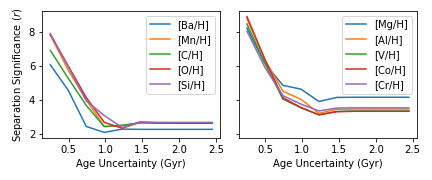
\includegraphics[width=\columnwidth]{figures/same_axis_r_age.png}
    \caption{Separation significance $r$ against age uncertainty (in Gyr) for all elements. These plots were made using data in the time-span between 4 and 5 Gyr after formation. So a 1 Gyr uncertainty is just over 20\% uncertainty. The five elements in the right-side plot have notably higher r-values than those in the left plot. The figure clearly demonstrates the age uncertainty at which we can become quite confident that we are observing two separate populations.}
    \label{fig:r_v_age}
\end{figure}

% This further motivates our second test of the influences of ages. Fig.~\ref{fig:r_v_age} shows each element plotted with r-value against age uncertainty (in Gyr). These particular plots were created using data between \SB{4 and 5 Gyr - have to be adjusted to stellar age}, which means that a 1 Gyr uncertainty is equivalent to just over 20\%. From these plots, we can see that there is a fair amount of variance between the elements. Regardless, it is clear that at an uncertainty of around 1.25 Gyr (or 25\%) the r-value begins to increase. At the next interval of around 0.75 Gyr (or 15\%) there is a very rapid increase in confidence. This informs us that ideally, we are striving for an uncertainty of less than 15\%, which is significantly lower than the uncertainties we are working with at the moment.

% \SB{I believe we should rather perform some MC simulations of relative abundance and age uncertainties. We can do that quite simple by multiplying the ages by a factor that is sampled from a normal distribution around 1 with a scatter value, e.g. 0.15 - is 0.15 corresponding to 15\% uncertainty?}

Fig.~\ref{fig:nihao_with_scatter}

\begin{figure*}
	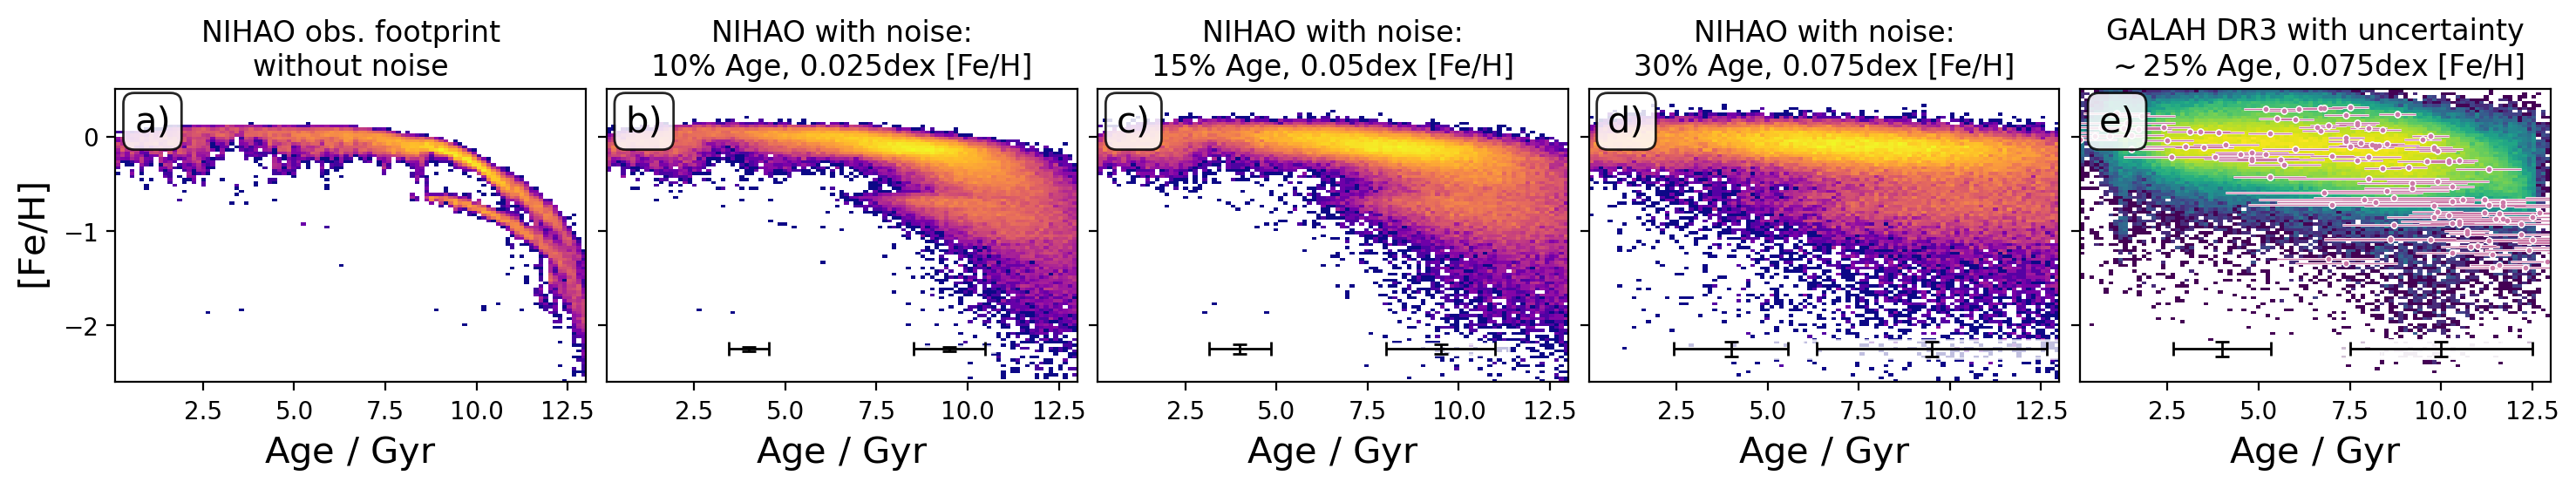
\includegraphics[width=\textwidth]{figures/nihao_with_scatter.png}
    \caption{
    \textbf{Comparison of age-metallicity relation for different scatter realisations for NIHAO simulations.}
    \textbf{Panel a)} show NIHAO without scatter, \textbf{panels b-e} show realisations of the same plot with increasingly more scatter sampling. \textbf{Panel f} show the GALAH DR3 age-metallicity relationship for comparison.
    }
    \label{fig:nihao_with_scatter}
\end{figure*}

% \textbf{Key Takeaways:} We can quantify the results and determine exactly what level of noise and age uncertainty is permissible to be able to separate the populations with 68\% and 95\% confidence. 

\subsection{Investigating the age-abundance sequences of the simulations}\label{sec:uncertainties}

Plotting elemental abundance vs age in Fig. \ref{fig:BaFetime} and \ref{fig:BaHtime} showed three distinct streams in the simulated plots. We explore these populations more closely here, and examine how these three populations appear in dynamical and chemical space as well. This is clearly laid out in Fig. \ref{fig:NaFe_MgMn_selection_Age_FeH_dissection}, showing the three population streams of the simulated galaxy in abundance-age plots in three distinct colours. These subsections are then considered in dynamical terms: considering where the stars lie in terms of galactic height against radius. We see that the in-situ stars (blue) are situated mostly around the Galactic plane, as expected. As we also expect, the population known to be accreted (red) has significantly more scatter in its spatial distribution, however the stars are still concentrated around the same plane. This is further the case when considering the third, probably accreted, stream (purple). There is too much intrinsic overlap between the populations to distinguish three separate streams of stars in dynamical space. \par 
This is similarly the case when considering two different abundance planes: an alpha element vs metallicity and [Mg/Mn] vs [Fe/H], as explored in observations in Sec. \ref{sec:feh_xfe} and \ref{sec:alfe_mgmn}. We expect the accreted bodies of stars to have notably lower abundances of alpha elements (REF), but again there is far too much chemical overlap between the populations to confidently separate the accreted from the in-situ based on alpha elements alone. Similarly, examining the [Mg/Mn] vs [Al/Fe] plots should demonstrate the difference between elements formed by SnII and Sn1a supernovae, as Mg is formed primarily in massive stars and returned to the ISM via SNeII \citep{Kobayashi2020} and Mn is generally produced by SNe1a explosions. Again, we can identify some distinct patterns of stars in this plane, but there is significant overlap. Studying Fig. \ref{fig:NaFe_MgMn_selection_Age_FeH_dissection} shows that we cannot rely on the chemical abundance planes created from simulation data to grant significant insight into accreted and in-situ populations, as there is too much intrinsic overlap to confidently separate them. \par 
\textbf{Key Takeaway:} There is too much intrinsic overlap in the dynamic and chemical properties of the accreted and in-situ populations identified in the simulation data to confidently distinguish different populations from these plots. 


%Selection sequences via age-[Fe/H] relation in Fig.~\ref{fig:sequences_in_age_feh}:

% \begin{align}
%     [Fe/H] > -0.2 \text{ or } \newline
%     ([Fe/H] > -1 \text{ and } 10^{\mathrm{[Fe/H]}+0.2}) \newline
% %    ((sim['Fe_H'] > -1.) & (13.80-sim['tform'] < 7)) |
% %    (10**(sim['Fe_H']+0.2) > 1.9 - 0.15*(13.40-sim['tform']))
% %)
% \end{align}

% Then look at their spatial extend in Fig.~\ref{fig:sequences_in_space} and their kinematic extend in Toomre diagrams (Fig.~\ref{fig:sequences_in_toomre})

% Toomre diagram of halo stars: \citet{Nissen2010} where UVW == VxVyVz or almost similarly VrVphiVz. Vphi traces azimuthal veloicity, which is an indicator of a stellar orbit's angular momentum (0 == no rotation with the stellar disk, high values == fast prograde rotation with the stellar disk, negative values == fast retrograde rotation against the stellar disk). The other dimension tells your something about the eccentricity (0 == ciruclar orbits, high values == highly eccentric)

% % \begin{figure}
% % 	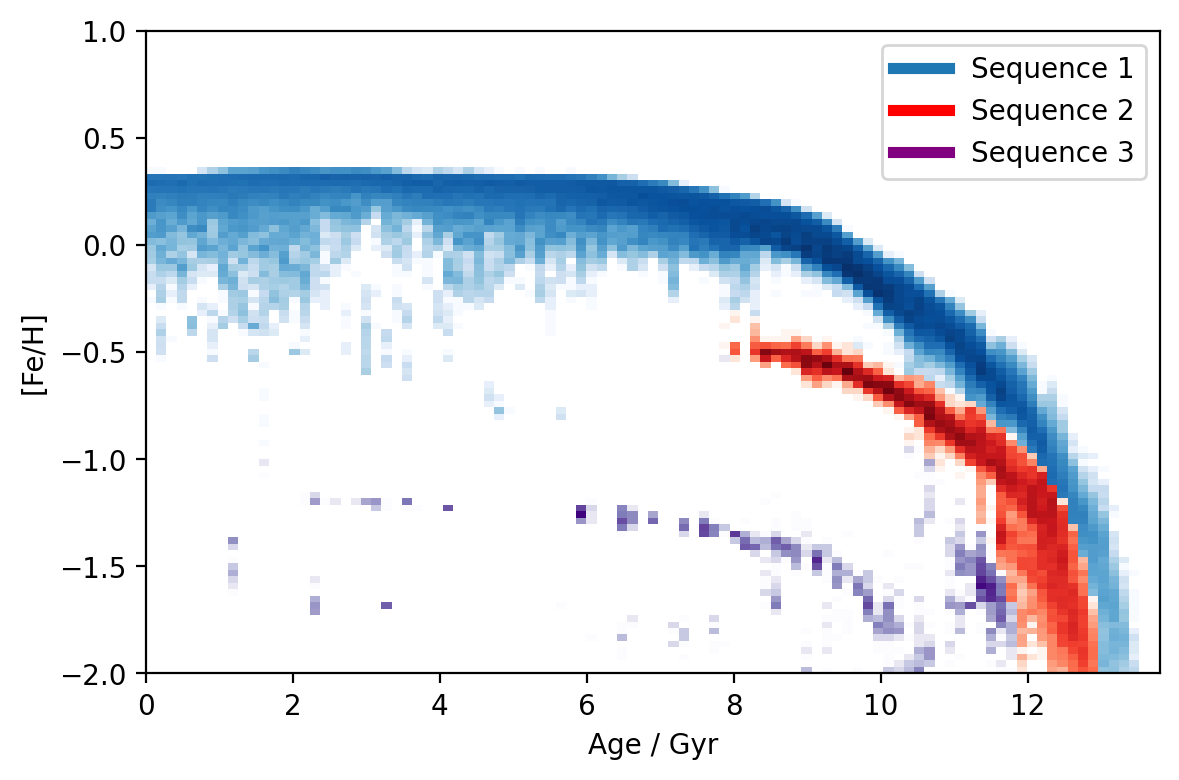
\includegraphics[width=\columnwidth]{figures/sequences_in_age_feh.png}
% %     \caption{Visualisation of selecting 3 different sequences in the simulated Age-[Fe/H] diagram.}
% %     \label{fig:sequences_in_age_feh}
% % \end{figure}

% % \begin{figure}
% % 	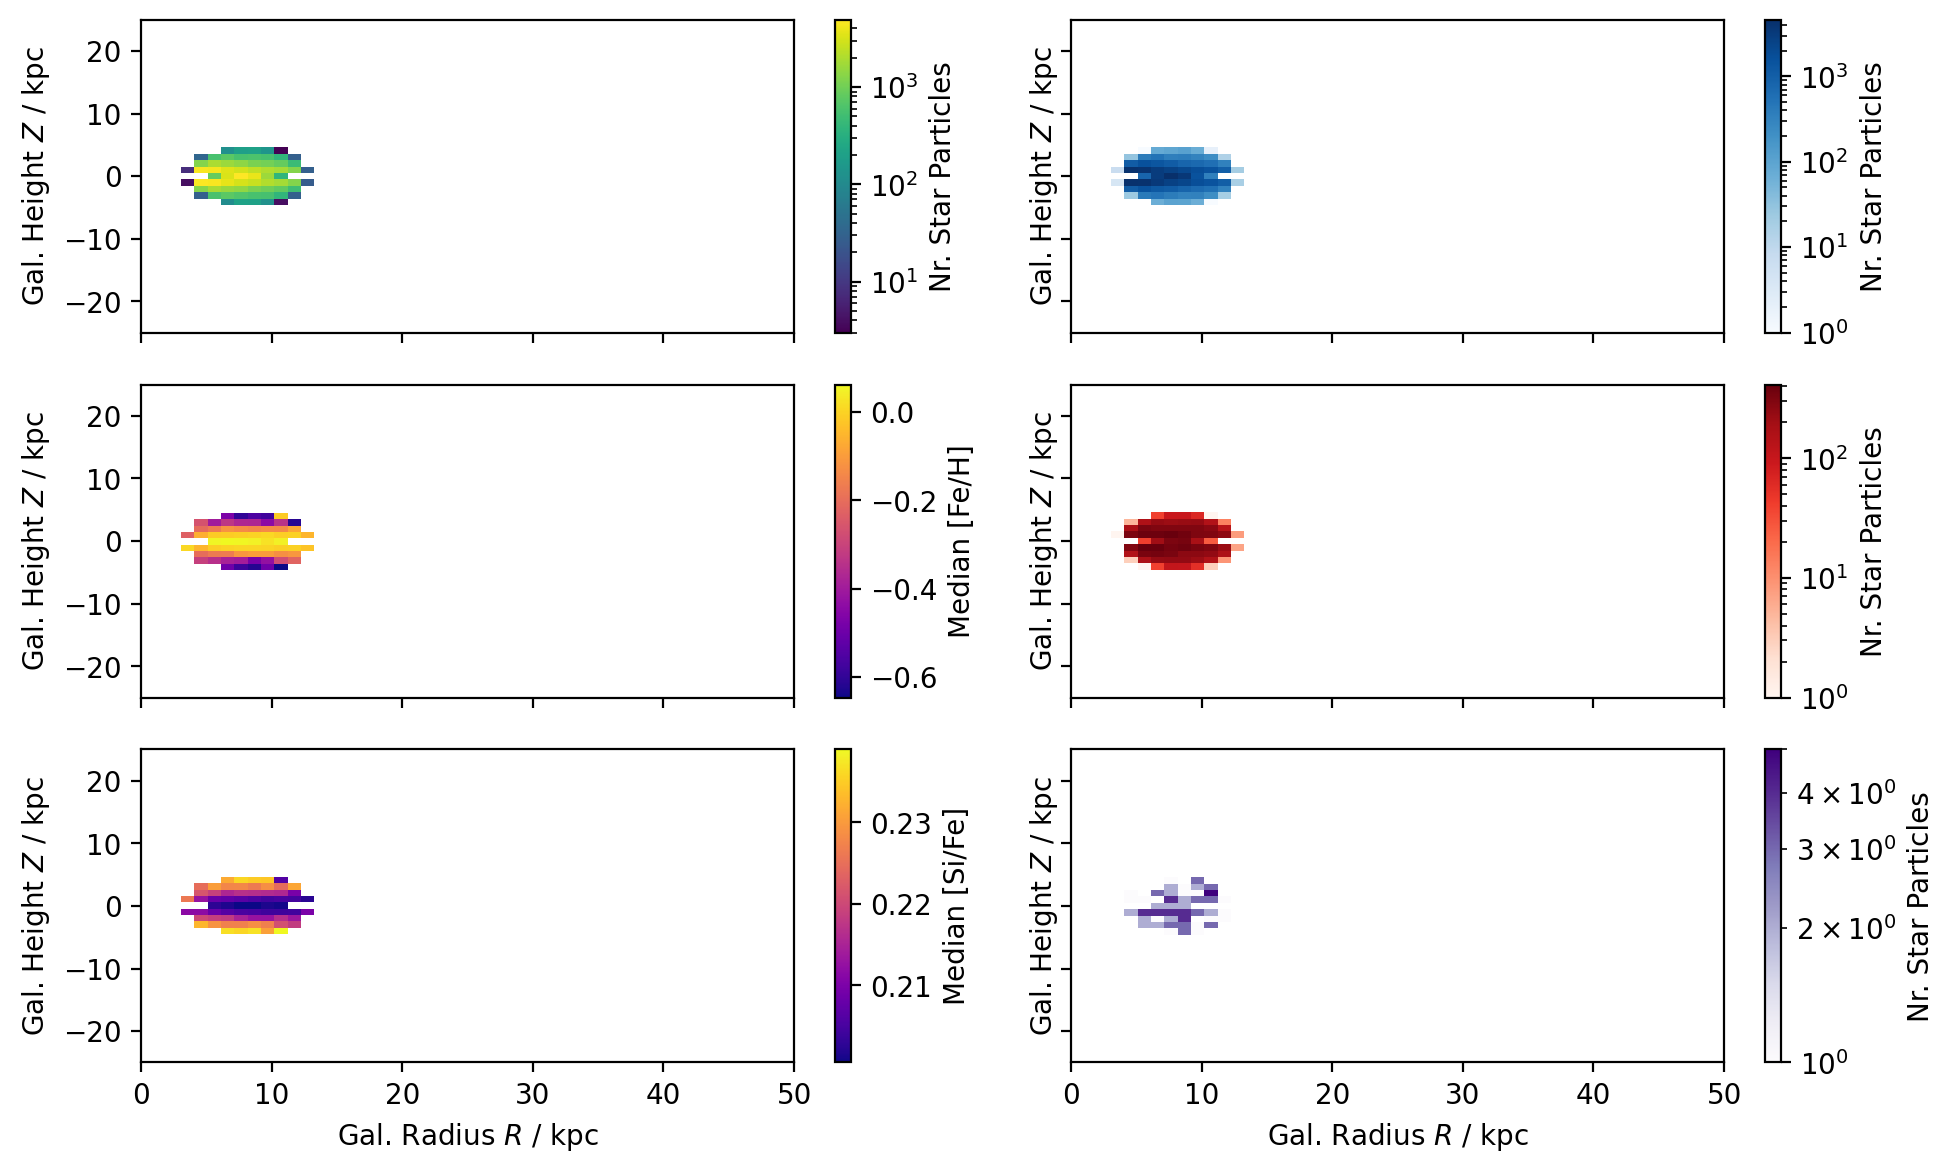
\includegraphics[width=\columnwidth]{figures/sequences_in_space.png}
% %     \caption{Spatial distribution of the full sample and its abundances (left) as well as of the sequences selected in Fig.~\ref{fig:sequences_in_age_feh}.}
% %     \label{fig:sequences_in_space}
% % \end{figure}

% % \begin{figure}
% % 	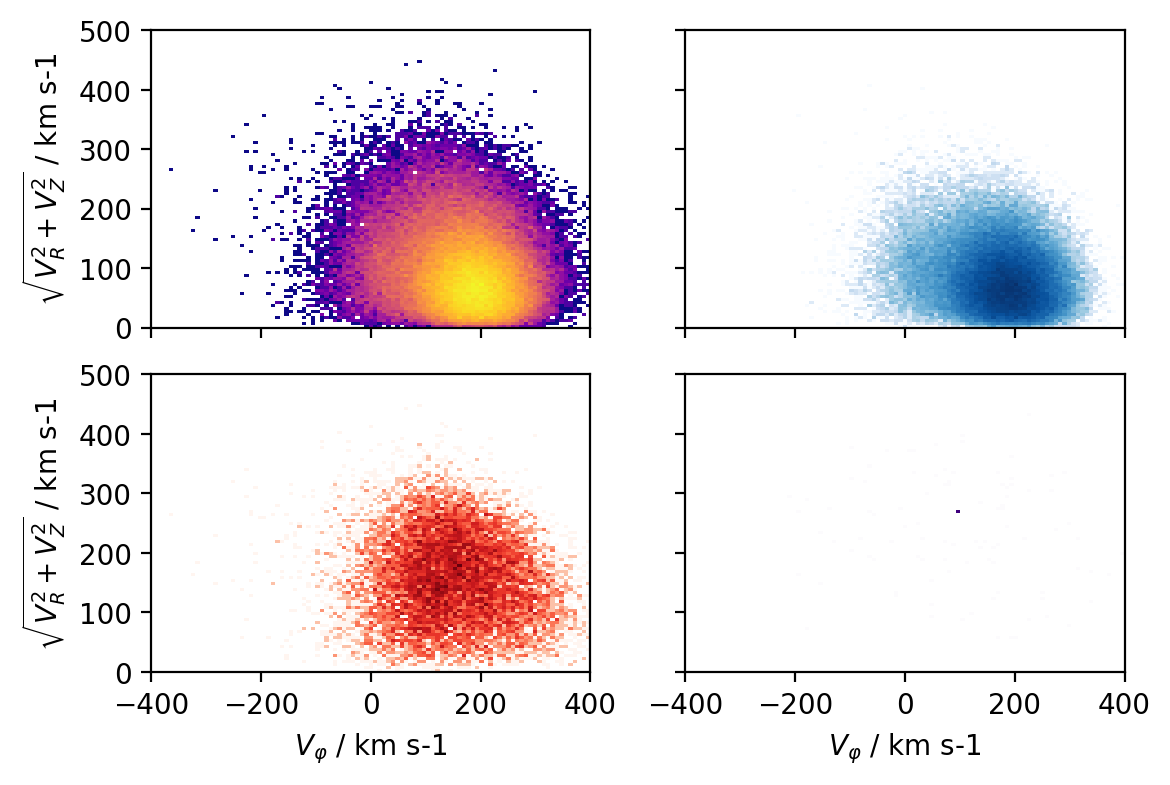
\includegraphics[width=\columnwidth]{figures/sequences_in_toomre.png}
% %     \caption{Velocity distribution in form of a Toomre diagram ($V_\phi$ vs. $\sqrt{V_R^2 + V_Z^2}$) of the full sample as well as of the sequences selected in Fig.~\ref{fig:sequences_in_age_feh}.}
% %     \label{fig:sequences_in_toomre}
% % \end{figure}

\subsection{The potential of age to clean chemical selections}

% Select stars in a rectangle locations of [Na/Fe] vs. [Mg/Mn] and then plot the ones with a below a certain Age-[Fe/H] relation in left panels and those above in the right panels of Fig.~\ref{fig:NaFe_MgMn_selection_Age_FeH_dissection}.

From the simulated galaxy, and the findings displayed in Fig \ref{fig:BaFetime}, \ref{fig:BaHtime} and \ref{fig:NaFe_MgMn_selection_Age_FeH_dissection}, we can apply our knowledge of how we expect accretion to appear in element vs abundance plots to 'clean' the observations, to an extent. We know that we expect to see (at least) two distinct streams in the [Fe/H] vs age plots. We are currently limited by very large age uncertainties in GALAH age measurements, so these populations are difficult to determine in our current observational plots (Figs. \ref{fig:BaFetime} and \ref{fig:BaHtime}). However, using the simulated plots to inform our expectations of the trends and substructure, we can explore the GALAH data more thoroughly. Expecting two distinct streams in age-abundance plots means we can correlate age-abundance  with abundance-abundance plots, to refine populations in chemical space. \par 
This is shown in Fig \ref{fig:NaFe_MgMn_selection_Age_FeH} where the different coloured sections correspond to increasingly large selections of stars in the [Mg/Mn] vs [Na/Fe] plane. We see that the smallest subset (red) has two clearly defined populations where we expect the accreted and in-situ stars to be. The significance and clarity of separation between the two populations decreases as the selection size increases (moving to the right across the figure). The blue subset, for example, shows no hint of two distinct populations. We can now determine how selective we need to be in the observational abundance-abundance plots in order to identify two clear populations. \par 
\textbf{Key Takeaway:} We can use the simulation abundance-age plots to clean our selection of chemical abundance plots from the observational data. 


\begin{figure*}
	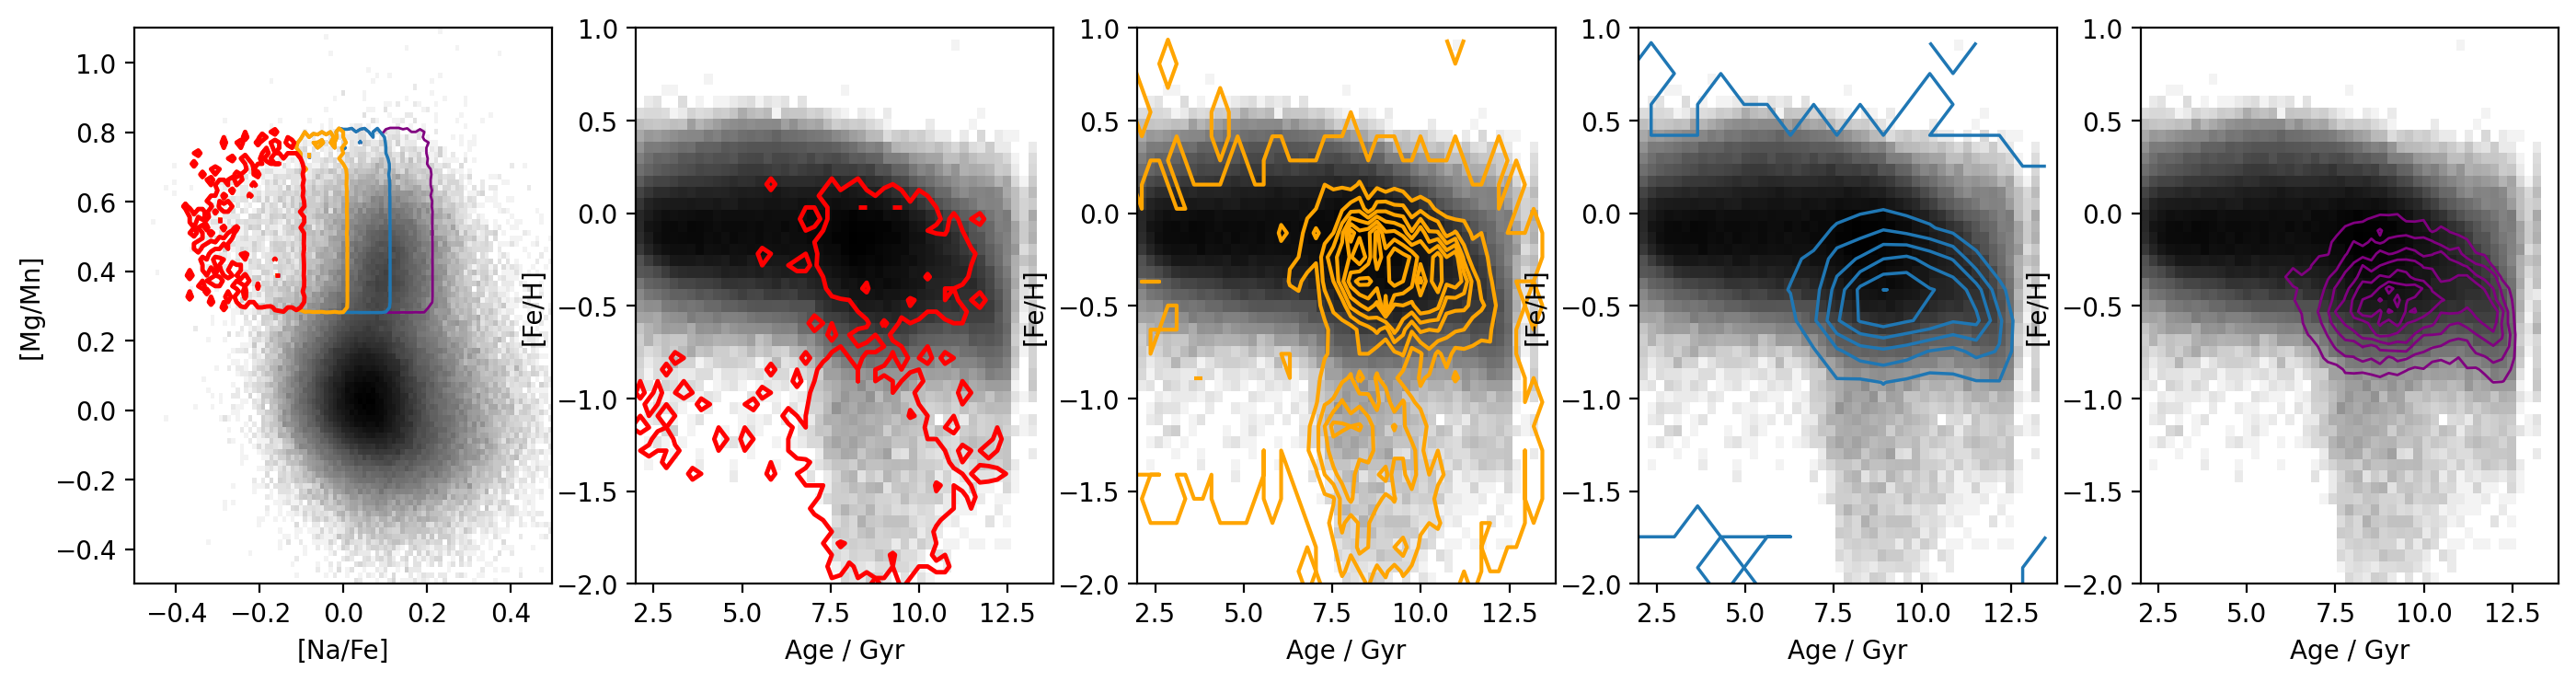
\includegraphics[width=\textwidth]{figures/NaFe_MgMn_selection_Age_FeH.png}
    \caption{Panel 1: The abundance plane of observed [Mg/Mn] vs [Na/Fe] showing four different (increasing in size) selections of stars. Each selection is then }
    \label{fig:NaFe_MgMn_selection_Age_FeH}
\end{figure*}




%%%%%%%%%%%%%%%%%%%%%%%%%%%%%%%%%%%%%%%%%%%%%%%%%%
\section{Discussion} \label{sec:discussion}
The initial motivation of this research was to create a variety of abundance planes and compare them using both the simulated and observed data to determine the best abundance-abundance plots for identifying substructure that could be representative of an accreted population of stars. Upon doing so, and observing very little distinct substructure in the simulated plots, these methods were deemed insufficient to confidently report any results. Due to the lack of potential observational uncertainties in the simulations, we expected to find significantly clearer substructure and distinct populations than had already been identified in observations \citep{Buder2022}. The fact that this wasn’t the case indicated a potential underlying problem in the theory behind this undertaking.  \par 
Beyond a lack of observational errors, one of the key advantages of the simulations is that we know the exact history of formation and accretion  of the simulated galaxy. Unfortunately, we do not yet have the same level of certainty surrounding our own Galaxy’s evolution. We know that the simulations are based on a merger event that occurred 5Gyr after formation, when a galaxy around $10e9 M_{\odot}$ merged with an in situ galaxy of around $10e10 M_{\odot}$. %These values that have been estimated to the order of magnitude by multiplying the number of star particles with their average stellar mass for each sequence of the simulation.
Although we do not know the exact sizes or times of accretion events in the Milky Way, the GSE is estimated to be between 108.7 and 109.85 $M_{\odot}$ (Helmi et al. 2018; Naidu et al. 2020), which highlights a possible discrepancy between the simulations and the observations. Even a small deviation in evolution could lead to vastly different outcomes, and could explain the discrepancy between observed substructure in the Milky Way, and the lack thereof in the simulated galaxy. Until we can be more confident regarding the history of our Milky Way, this will remain a significant shortcoming of using simulations in this way. \par 
The lack of reportable findings from comparing abundance-abundance planes led to a shift in focus. As discussed in Sec. \ref{sec:intro}, one of the key advantages to chemical tagging is the unchanging nature of stellar chemistry over time. This means that a star’s current chemical make-up is indicative of the time and place that it was born. Therefore plotting elemental abundance over time was hypothesised as a good indicator of accretion, as populations of different chemistry should emerge as the galaxy evolves. This was plotted and analysed in Section \ref{sec:Age-abundance}. We see three clear populations emerge in the simulations, highlighted in Fig \ref{fig:NaFe_MgMn_selection_Age_FeH_dissection}. \par 
Again, it is important to note that the simulated galaxy may have different characteristics to our own Galaxy. As discussed, there are two clear streams that have been attributed as accreted and in situ, based on the assumption that the accreted stars would have been born in a smaller galaxy with less massive stars and therefore lower element abundances. This clarity occurs because we know the sizes of the two galaxies that merged. Depending on the size of the real merger in the Milky Way, there could be significantly more overlap between the accreted and in situ populations if the merger was more massive. Even within the simulated data, we see significant overlap in the kinematic and chemical characteristics of the three separate streams, which is clear in Fig \ref{fig:NaFe_MgMn_selection_Age_FeH_dissection}. This indicates that within the simulated data, and potentially the real Milky Way, there may be significant uncertainty in distinguishing between the accreted and in situ populations, using the dynamic or chemical information. \par 
However, there is potential in using the simulations to ‘clean up’ the observational data. In assessment of Fig. \ref{fig:BaFetime} and \ref{fig:BaHtime}, we see large amounts of scatter in the observations. However, there is a hint of an overdensity toward the bottom right of the plot, which could be indicative of an accreted population. Applying the quality cute provided with the GALAH data had little effect on the clarity of this overdensity, but with better quality cuts, more time and expertise- and better data- this ‘hint’ could start looking more like what is shown in the observations.\par 
I would strongly recommend that similar research is performed with other cosmological simulations, preferably with varied chemistry and formation histories. This would enable researchers to observe exactly how different variables in the simulation affect outcomes. More importantly, the research was limited by the uncertainties present in the observations, especially in the ages. If the error margins corresponding to age measurements can be drastically reduced, we have found that plotting element abundance over age holds significant potential for the identification of accreted stars. \par 




% This project began with the intention of creating a variety of abundance planes and comparing both simulation and observation data to identify substructure within the plots that was representative of accreted stars. Upon doing so, and observing very little clear substructure in the simulation plots, these plots were deemed insufficient to confidently report any results. There are two major advantages to using cosmological simulations. The first of these is that there are no measurement uncertainties to consider, which should produce clear and accurate plots with no doubt of extrinsic scatter. This means that although some distinct populations were seen in the observational plots, the absence of clarity in the simulation-based plots questions that measurement uncertainties are the main difference between observations and simulations.   
% Beyond measurement uncertainties, the second key advantage to the cosmological simulations is that the exact, detailed formation history of the simulated galaxy is known. Knowing what merged with the galaxy and when is crucial in identifying accretion, but this is knowledge that we don't possess to a desirable level for the Milky Way in reality. This poses a challenge in how we can use the cosmological simulations, as we have no guarantee that we are simulating the evolution of the Milky Way. It may also contribute to the discrepancies between the simulations and observations. If the simulations are replicating even a slightly different galaxy, this could explain the lack of clear substructure that we can see in observations. We know that the simulations are based on a merger event that occurred 5Gyr after formation, when a galaxy around $10^9 M_{\odot}$ merged with an in situ galaxy of around $10^{10} M_{\odot}$, values that have been estimated to the order of magnitude by multiplying the number of star particles with their average stellar mass for each sequence of the simulation. Although we do not know the exact sizes or times of accretion events in the Milky Way, the GSE is estimated to be between $10^{8.7}$ and $10^{9.85}\,M_{\odot}$ \citep{Helmi2018,Naidu2020}, which highlights a possible discrepancy between the simulations and the observations. Until we have a more exact understanding of the formation history of the Milky Way, we cannot ensure these simulations are accurate, which is an important caveat to keep in mind.   
% From this, the focus of the project underwent a shift, looking instead at other observables beyond chemical abundance that could be used and plotted to identify accreted stars. As Section \ref{sec:intro} makes clear, one of the key advantages to chemical tagging is the unchanging nature of stellar chemistry over time, meaning that a star's current chemical make-up is indicative of the time and place that it was born. Therefore, plotting elemental abundance over time was hypothesised as a good indicator of accretion, where separate populations should be clear. This was plotted and analysed in Section \ref{sec:ageabundance}, and found that indeed there are two clear stellar populations in the simulation data, indicative of accreted and in situ stars, that were not seen in the observational data due to measurement uncertainties.  
% Despite this positive outcome, it is still important to address the possibility of intrinsic overlap between accreted and in situ stars. As discussed, there are two clear streams that have been attributed as accreted and in situ, based on the assumption that the accreted stars would have been born in a smaller galaxy with less massive stars and therefore lower element abundances. This clarity occurs because we know the sizes of the two galaxies that merged. Depending on the size of the real merger in the Milky Way, there could be significantly more overlap between the accreted and in situ populations if the merger was more massive. This means that from the abundance-age plots alone, it is harder to tell if the situ stream is completely made up of Milky Way-born stars. 

% A further recommendation is that it would be worth putting effort into further analysing Fig.~\ref{fig:BaHtime}. Despite the massive amount of scatter in the observations, when Ba was plotted in a ratio with H, there appears to be a hint of an overdensity toward the bottom right of the plot, which could indicate an accreted population. Applying the quality cuts provided in the GALAH data had little effect on how clear this overdensity appears. It is beyond the scope of this project, but with better quality cuts, more time and expertise - and better data, this 'hint' could start indicating something that looks more like the simulations, which would further confirm that plots of elements against time are worth pursuing.  
% This project was limited by a number of variables, one of which was simply the number of elements that could be analysed. The caveat for an element to be used in this project was that it had to be included in the datasets of both the simulations, and the GALAH survey. This reduced the total number of elements to just ten. Moreover, although there were quite a number of iron-peak elements, the remaining element groups only contained two options, with Ba being the only neutron capture element. This reduced the ability to make in-depth assessments based on element groups, as the sample size was simply not large enough to consider any trends with certainty. To this end, it could be worth pursuing other datasets with a different choice of elements.  
% Moreover, I would strongly recommend similar research is performed with other cosmological simulations, preferably with varied chemistry and formation histories. This would enable researchers to observe exactly how different variables in the simulation affect outcomes. 
% The main observational limitation to this project was simply measurement uncertainties, particularly in ages. If the errors corresponding to age measurements can be drastically reduced, plotting elements over time has the potential to be a great diagnostic tool for accreted stars. 


%%%%%%%%%%%%%%%%%%%%%%%%%%%%%%%%%%%%%%%%%%%%%%%%%%

%%%%%%%%%%%%%%%%%%%%%%%%%%%%%%%%%%%%%%%%%%%%%%%%%%
\section{Conclusions}
\label{sec:conc}

The aim of this paper was to determine the best diagnostic plots for identifying accreted stars in the Milky Way, through comparison of a cosmological simulation from the NIHAO suite and data from the GALAH survey. 

\SB{Absence of features does not mean that they are not present! We initially thought that the chemical abundance planes of the simulation possessed too much intrinsic overlap to be useful to this particular endeavour. But that was based on diagnostic plots for the whole galaxy! Sec.~\ref{sec:location}}

Plotting elemental abundances against age instead proved fruitful. Very distinct stellar streams representing accreted and in-situ stars were clear in the simulated age plots that were not apparent in the observation-based plots, due to the massive uncertainties that come with the probabilistic nature of estimating stellar ages through isochrone fitting. We found therefore that the best plots from the simulations to identify accretion were elemental abundances, relative to H, against stellar age. \par 
Adding noise to the simulated data suggests that we will be able to more confidently tell apparent accreted structures once we can determine ages within an uncertainty of 15\% and can measure elemental abundances [X/H] of accreted structures as good as $\sigma_{obs}\sim0.40$ dex. We determined that although there were three clear population streams apparent in the simulated data, significant overlap appeared when these were plotted in terms of dynamical and chemical properties. Instead, we have shown how the simulations may be used to clarify the observational plots. We conclude that this study holds exciting prospects for the future of our understanding of accretion in the Milky Way. As our observational data continues to improve, we will increase our confidence in recognising accreted stars in our own Galaxy. 

\SB{NOTE TO OURSELVES: We see this interesting prediction of high [Ba/Fe] for the youngest accreted stars in both observations and simulations! That is quite remarkable and can maybe help us to study the influence of AGB stars in the metal-poor regime?!}

\SB{Future Analysis:}
\begin{itemize}
\item Age and abundance precision for different 25ish NIHAO sims
\item Age and abundance precision for different yields
\end{itemize}

\SB{Selection does not affect the age-metallicity relations, but definitely the [Al/Fe] vs. [Mg/Mn] plane! Just because don't something in one the planes does not mean it's not there!}


\SB{These observations of stellar and gaseous components complement the advancements from the modelling perspective, where recent studies have found significant impacts of massive mergers on the cold gas metallicity gradients \citep{Buck2023}. \citet{Buck2023} analyse the impact of mergers on the abundance gradients for example in the age-metallicity relation. Also cite Agertz etc.}

% The aim of this project was to determine suitable diagnostic plots for identifying accreted stars in our Milky Way, through comparison of a cosmological simulation from the NIHAO suite with data from the GALAH survey. The major take-aways from this undertaking were:
% \begin{itemize}
% \item Chemical abundance planes of the simulations possess too much intrinsic overlap to be useful to this particular research project. 
% \item Plotting elemental abundances against age however, proved fruitful, with very distinct streams representing accreted and in situ populations appearing in the simulation data. These clear streams were not apparent in the observation-based plots, as a result of massive uncertainties that come with the probabilistic nature of estimating stellar ages through isochrone fitting.
% \item Elemental abundances as relative to H (rather than Fe) produced more significant separations between in-situ and accreted sequences as a function of stellar age.
% \item Our tests of adding noise to simulated data suggest, that we will be able to more easily tell apart accreted structures, once we undergo a critical age uncertainty of 15\% and can measure elemental abundances [X/H] of accreted structures as good as $\sigma_\text{obs} \sim 0.40\,\mathrm{dex}$.
% \end{itemize}

% Overall, reducing uncertainties in ages is a difficult task that may take a long time, but as data and techniques continue to improve these values, there is much potential in using plots of elemental abundances over time as a diagnostic tool for accreted stars.

\section*{Acknowledgements}

We acknowledge the traditional owners of the land on which the AAT and ANU stand, the Gamilaraay, the Ngunnawal and Ngambri people. We pay our respects to elders past, present, and emerging and are proud to continue their tradition of surveying the night sky in the Southern hemisphere.

This work was supported by the Australian Research Council Centre of Excellence for All Sky Astrophysics in 3 Dimensions (ASTRO 3D), through project number CE170100013.

SB acknowledges support from the Australian Research Council under grant number DE240100150.

TB acknowledges support from the European Research Council under ERC-CoG grant CRAGSMAN-646955.

\section*{Facilities}

\textbf{AAT with 2df-HERMES at Siding Spring Observatory:}
The GALAH Survey is based data acquired through the Australian Astronomical Observatory, under programs: A/2013B/13 (The GALAH pilot survey); A/2014A/25, A/2015A/19, A2017A/18 (The GALAH survey phase 1), A2018 A/18 (Open clusters with HERMES), A2019A/1 (Hierarchical star formation in Ori OB1), A2019A/15 (The GALAH survey phase 2), A/2015B/19, A/2016A/22, A/2016B/10, A/2017B/16, A/2018B/15 (The HERMES-TESS program), and A/2015A/3, A/2015B/1, A/2015B/19, A/2016A/22, A/2016B/12, A/2017A/14, (The HERMES K2-follow-up program). This paper includes data that has been provided by AAO Data Central (datacentral.aao.gov.au).

\textbf{\Gaia: } This work has made use of data from the European Space Agency (ESA) mission \Gaia (\url{http://www.cosmos.esa.int/gaia}), processed by the \Gaia Data Processing and Analysis Consortium (DPAC, \url{http://www.cosmos.esa.int/web/gaia/dpac/consortium}). Funding for the DPAC has been provided by national institutions, in particular the institutions participating in the \Gaia Multilateral Agreement. 

\textbf{Other facilities:} This publication makes use of data products from the Two Micron All Sky Survey \citep{Skrutskie2006} and the CDS VizieR catalogue access tool \citep{Vizier2000}.

\section*{Software}

The research for this publication was coded in \textsc{python} (version 3.7.4) and included its packages
\textsc{astropy} \citep[v. 3.2.2;][]{Robitaille2013,PriceWhelan2018},
\textsc{corner} \citep[v. 2.0.1;][]{corner},
\textsc{IPython} \citep[v. 7.8.0;][]{ipython},
\textsc{matplotlib} \citep[v. 3.1.3;][]{matplotlib},
\textsc{NumPy} \citep[v. 1.17.2;][]{numpy},
\textsc{pynbody} \citep[v. 1.1.0;][]{pynbody},
\textsc{scipy} \citep[version 1.3.1;][]{scipy},
\textsc{sklearn} \citep[v. 0.21.3;][]{scikit-learn},
We further made use of \textsc{topcat} \citep[version 4.7;][]{Taylor2005};

%%%%%%%%%%%%%%%%%%%%%%%%%%%%%%%%%%%%%%%%%%%%%%%%%
\section*{Data Availability}

The observational data used for this study is published by \citet{Buder2021} and can be accessed publicly via \url{https://docs.datacentral.org.au/galah/dr3/overview/}

All code to reproduce the analysis and figures can be accessed via \url{https://github.com/svenbuder/Accretion_Clues_ObsSim}.

Simulated data can be retrieved from the authors upon reasonable request.

%%%%%%%%%%%%%%%%%%%% REFERENCES %%%%%%%%%%%%%%%%%%

% The best way to enter references is to use BibTeX:
\bibliographystyle{mnras}
\bibliography{bib} % if your bibtex file is called example.bib

%%%%%%%%%%%%%%%%%%%%%%%%%%%%%%%%%%%%%%%%%%%%%%%%%%
%%%%%%%%%%%%%%%%% APPENDICES %%%%%%%%%%%%%%%%%%%%%

% \newpage
% \appendix

%%%%%%%%%%%%%%%%%%%%%%%%%%%%%%%%%%%%%%%%%%%%%%%%%%

% Don't change these lines
\bsp	% typesetting comment
\label{lastpage}
\end{document}

% End of mnras_template.tex
